%%% Local Variables:
%%% TeX-master: "main"
%%% End

\documentclass[
12pt, % The default documnt font size, optins: 10pt, 11pt, 12pt
% oneside, % Two side (alterating margins) for binding by default,
% uncomment to switch to one side
english, % ngerman for German
doublespacing, % Single line spacing, alternatives: onehalfspacing or dBoublespacing#
% draft, % Uncomment to enable draft mode (no pictures, no links, overfull hboxes indicated)
% nolistspacing, % If the document is onehalfspacing or doublespacing, uncomment this to set spacing in lists to single
% liststotoc, % Uncomment to add the list of figures/tables/etc to the table of contents
%toctotoc, % Uncomment to add the main table of contents to the table of contents
%parskip, % Uncomment to add space between paragraphs
%nohyperref, % Uncomment to not load the hyperref package
headsepline, % Uncomment to get a line under the header
chapterinoneline, % Uncomment to place the chapter title next to the
                  % number on one line
% consistentlayout, % Uncomment to change the layout of the declaration, abstract and acknowledgements pages to atch the default layout
]{MastersDoctoralThesis} % The class file specifying the document structure
\usepackage[utf8]{inputenc} % Required for inputting international characters
\usepackage[T1]{fontenc} % Output font encoding for international characters
\usepackage{mathpazo} % Use the Palatino font by default

%% author year style
\usepackage[backend=bibtex,style=authoryear,natbib=true]{biblatex}
% uncomment to make author names italic
% \renewcommand{\mkbibnamelast}[1]{\mkbibemph{#1}}
%% author names in small capitals 
\renewcommand{\mkbibnamelast}[1]{\small{\textsc{#1}}}

%% numerics numbered by appearance 
%\usepackage[backend=bibtex, style=numeric,sorting=none]{biblatex} % Use the bibtex

%\usepackage[backend=bibtex,style=alphabetic]{biblatex}

\addbibresource{example.bib} % The filename of the bibiography
\usepackage{rotating}
\usepackage[autostyle=true]{csquotes} % Required to generate language-dependent quotes in the bibliography
\usepackage{listings}
\usepackage{float}
\usepackage{xcolor}
\usepackage{mathtools}
\usepackage{enumerate}
\usepackage{longtable}
\usepackage{tikz}
\usetikzlibrary{shapes.geometric, arrows}
\tikzstyle{startstop} = [rectangle, rounded corners, minimum width=3cm, minimum height=1cm,text centered, draw=black, fill=red!30]
\tikzstyle{io} = [trapezium, trapezium left angle=70, trapezium right angle=110, minimum width=3cm, minimum height=1cm, text centered, draw=black, fill=blue!30]
\tikzstyle{process} = [rectangle, minimum width=3cm, minimum height=1cm, text centered, draw=black, fill=orange!30]
\tikzstyle{decision} = [diamond, minimum width=3cm, minimum height=1cm, text centered, draw=black, fill=green!30]
\tikzstyle{arrow} = [thick,->,>=stealth]



\makeatletter
\renewcommand*\env@matrix[1][c]{\hskip -\arraycolsep
  \let\@ifnextchar\new@ifnextchar
  \array{*\c@MaxMatrixCols #1}}
\makeatother

\pagenumbering{alph}

% \definecolor{codegreen}{rgb}{0,0.6,0}
% \definecolor{codegray}{rgb}{0.5,0.5,0.5}
% \definecolor{codepurple}{rgb}{0.58,0,0.82}
% \definecolor{backcolour}{rgb}{0.95,0.95,0.92}

\definecolor{codegreen}{gray}{0.3}
\definecolor{codegray}{gray}{0.5}
\definecolor{codepurple}{gray}{0.58}
\definecolor{backcolour}{gray}{1}
 
\lstdefinestyle{mystyle}{
  backgroundcolor=\color{backcolour},  
  commentstyle=\color{codegreen},
  keywordstyle=\color{codegreen},
  numberstyle=\tiny\color{codegray},
  stringstyle=\color{codepurple},
  basicstyle=\ttfamily\footnotesize,
  breakatwhitespace=false,     
  breaklines=true,         
  captionpos=b,          
  keepspaces=true,         
  numbers=left,          
  numbersep=5pt,         
  showspaces=false ,        
  showstringspaces=false,
  showtabs=false,        
  tabsize=2
 }
\lstset{style=mystyle}
% ------------------------------------------------------------------------------
%	MARGIN SETTINGS
% ----------------------------------------------------------------------------

\geometry{
  paper=a4paper, % Change to letterpaper for US letter
  inner=3cm, % Inner margin
  outer=2.5cm, % Outer margin
  bindingoffset=.5cm, % Binding offset
  top=1.5cm, % Top margin
  bottom=1.5cm, % Bottom margin
  % showframe, % Uncomment to show how the type block is set on the page
}
%----------------------------------------------------------------------------------------
%	THESIS INFORMATION
%----------------------------------------------------------------------------------------
\thesistitle{Quantitative genetics from genome assemblies to neural network aided omics-based prediction of complex traits} % Your thesis title 

\author{Jan Alexander \textsc{Freudenthal}} % Your name, this is used in the title page and abstract, print it elsewhere with \authorname
\addresses{} % Your address, this is not currently used anywhere in the template, print it elsewhere with \addressname
\subject{Biological Sciences} % Your subject area, this is not currently used anywhere in the template, print it elsewhere with \subjectname
\keywords{} % Keywords for your thesis, this is not currently used anywre in the template, print it elsewhere with \keywordnames
\university{\href{http://www.university.com}{Julius-Maximilians Universit\"{a}t W\"{u}rzburg}}
%\univname
\department{\href{http://department.university.com}{GSLS}} 
\group{\href{http://researchgroup.university.com}{Research group for evolutionary genomics}}
%\groupname
\usepackage{amsmath}

\begin{document} 
\frontmatter % Use roman page numbering style (i, ii, iii, iv...) for the pre-content pages

\pagestyle{plain} 


\begin{titlepage}
  \begin{center}
    {\scshape\Large
       \univname\par}\vspace{1.0cm}
     \includegraphics[height=0.2\textheight,width=0.35\textwidth]{wappen}
     
    \vspace{1.0cm}
    {\color{mdtRed}\Large \ttitle\par}
    \vspace{1.0cm}
    \thesistitle{Quantitative Genetik von Genomassemblierungen bis zur genomischen Vorhersage von ph\"{a}notypischen Merkmalen mit Hilfe von künstlichen neuronalen Netzwerken}
    {\color{mdtRed}\Large \ttitle\par}
    \vspace{1.0cm}
    Doctoral Thesis at the Graduate School of Life Sciences \\
    Section Integrative Biology \\
    submitted by \\
    \vspace{1.0cm}
    \color{mdtRed}{\Large\authorname} \\
    \vspace{1.0cm}
    \color{black}from
    \textbf{L\"{u}beck, Schleswig-Holstein, Germany}
    
    
  \end{center}
  \newpage
  
  \vspace{.1\textheight}
  \textbf{Submitted on:} \dotfill\\
  
  \vspace{.1\textheight}
  \begin{centering}
    {\Large\textbf{Members of the Thesis Committee:}} \\
      \vspace{.1\textheight}
      {\Large
      \textbf{Chairperson: }\textit{Prof. Thomas Schmitt} \\
      \textbf{Primary Supervisor: }\textit{Prof. Arthur Korte} \\
      \textbf{Supervisor (Second):  }\textit{Prof. J\"{o}rg Schultz } \\
      \textbf{Supervisor (Third):  }\textit{Prof. Thomas Dandekar} \\
      }
    \end{centering}
    \vspace{0.2\textheight}
    \noindent
    \textbf{Date of Public Defence:} \dotfill \\
    \textbf{Date of Receipt of Certificates:}\dotfill
  
  
\end{titlepage}

%----------------------------------------------------------------------------------------
%	DECLARATION PAGE
%----------------------------------------------------------------------------------------

\begin{declaration}
  \noindent
  {\LARGE\textbf{Affidavit}} \\
  \noindent
  I hereby confirm that my thesis entitled \textit{``Quantitative genetics -
  from genome assemblies to neural network aided omics based
  prediction of complex traits''} is the result of my own work. I did not
  receive any help or support from commercial consultants. All sources
  and  or materials applied are listed and specified in the thesis.
  Furthermore, I confirm that this thesis has not yet been submitted
  as part of another examination process neither in identical nor in
  similar form.

  \vspace{0.1\textheight}
  \noindent
  {\LARGE\textbf{Eidesstattliche Erkl\"{a}rung}}\\
  \noindent
  Hiermit erkläre ich an Eides statt, die Dissertation mit dem Titel \textit{``Quantitative Genetik von Genomassemblierungen bis zur genomischen Vorhersage von ph\"{a}notypischen Merkmalen mit Hilfe von künstlichen neuronalen Netzwerken''} 
  eigenst\"{a}ndig, d.h. insbesondere selbst\"{a}ndig und ohne Hilfe eines
  kommerziellen Promotionsberaters, angefertigt und keine anderen als
  die von mir angegebenen Quellen und Hilfsmittel verwendet zu haben.
  Ich erkl\"{a}re außerdem, dass die Dissertation weder in gleicher noch
  in \"{a}hnlicher Form bereits in einem anderen Pr\"{u}fungsverfahren
  vorgelegen hat.
\addchaptertocentry{Affidavit} % Add the declaration to the table of contents
\end{declaration}
\newpage

%\cleardoublepage

%----------------------------------------------------------------------------------------
%	QUOTATION PAGE
%----------------------------------------------------------------------------------------

\vspace*{0.2\textheight}

\noindent\enquote{\itshape Wit beyond measure is man's greatest treasure}\bigbreak

\hfill Rowena Rawenclaw

%----------------------------------------------------------------------------------------
% ABSTRACT PAGE
%----------------------------------------------------------------------------------------

%----------------------------------------------------------------------------------------
%	ACKNOWLEDGEMENTS
%----------------------------------------------------------------------------------------

\begin{acknowledgements}
   \addchaptertocentry{Acknowledgments} % Add the acknowledgements to the table of contents
   \noindent
   Thanks, to Prof. Arthur Korte for hiring me and the opportunity to conduct research and write this thesis in his group, as well as the invaluable help. \\
   Thanks, to Arthur, Prof. Jörg Schultz and Prof. Thomas Dandekar for the supervision and being part of the thesis committee. \\
   Thanks, to Prof. Thomas Schmitt for being the chairperson of the thesis committee. \\
   Thanks, to the co-authors of the chloroplast benchmarking project: Niklas Terhoeven, Simon Pfaff, Markus Ankenbrand and Frank Förster. \\
   Thanks, to the co-authors of the GWAS-Flow project: Markus Ankenbrand, Dominik Grimm and of course Arthur. \\
   Thanks, to the students who assisted in the genomic selection projects: Laura Steinmann, Roman Saiz and Florens Fischer as well as the other collaborators Markus Ankenbrand and Torsten Pook. \\
   Thanks, to the German Federal Ministry of Education and Research (BMBF) and the German
   tax payers for funding the MAZE project within the scope of the funding initiative
   “Plant Breeding Research for the Bioeconomy” (Funding ID: 031B0195). \\
   Thanks, to the MAZE project partners for the great collaboration in the past three years. \\
   And lastly, thanks to everyone at the CCTB for creating a great working environment. \\
\end{acknowledgements}


% \begin{abstract}
%   \addchaptertocentry{Abstract} % Add the abstract to the table of contents
%   \noindent
%    \vspace{10em}

% \newpage
% \noindent
% bnisse im Gesamtkontext der quantitativen Genetik beleuchtet.

% \end{abstract}

%----------------------------------------------------------------------------------------
%	LIST OF CONTENTS/FIGURES/TABLES PAGES
%----------------------------------------------------------------------------------------

\tableofcontents % Prints the main table of contents
\addcontentsline{toc}{chapter}{Table of contents}

\listoffigures % Prints the list of figures
\addcontentsline{toc}{chapter}{List of figures}

\listoftables % Prints the list of tables
\addcontentsline{toc}{chapter}{List of tables}
%----------------------------------------------------------------------------------------
%	ABBREVIATIONS
%----------------------------------------------------------------------------------------

\begin{abbreviations}{ll} % Include a list of abbreviations (a table of two columns)
  \addchaptertocentry{List of Abbreviations}
  \textbf{Adadelta} & \textbf{Ada}ptive \textbf{delta}                                                             \\
  \textbf{Adagrad}   & \textbf{Ada}ptive \textbf{Grad}ient Algorithm                                                \\
  \textbf{Adam}      & \textbf{Ada}ptive \textbf{M}oment estimation                                                 \\
  \textbf{ANN}       & \textbf{A}rtificial \textbf{N}eural \textbf{N}etwork                                         \\
  \textbf{API}       & \textbf{A}pplication \textbf{P}rogramming \textbf{I}nterface                                 \\
  \textbf{AUC}       & \textbf{A}rea \textbf{U}nder the \textbf{C}urve                                              \\
  \textbf{BL}        & \textbf{B}ayesian \textbf{Lasso}                                                             \\
  \textbf{BLUE}      & \textbf{B}est \textbf{L}inear \textbf{U}nbiased \textbf{E}stimator                           \\
  \textbf{BLUP}      & \textbf{B}est \textbf{L}inear \textbf{U}nbiased \textbf{P}redictor                           \\
  \textbf{bp}        & \textbf{B}ase \textbf{P}air                                                                  \\
  \textbf{BRR}       & \textbf{B}ayesian \textbf{R}idge \textbf{R}egression                                         \\
  \textbf{CPU}       & \textbf{C}ore \textbf{P}rocessing \textbf{U}nit                                              \\
  \textbf{DH}        & \textbf{D}oubled \textbf{H}aploid                                                            \\
  \textbf{DNA}       & \textbf{D}eoxyribo\textbf{N}ucleic \textbf{A}cid                                             \\
  \textbf{DNA}       & \textbf{R}ibo\textbf{N}ucleic \textbf{A}cid                                                  \\
  \textbf{EMMA}      & \textbf{E}fficient \textbf{M}ixed \textbf{M}odel \textbf{A}ssociations                       \\
  \textbf{FDR}       & \textbf{F}alse \textbf{D}iscovery \textbf{R}ate                                              \\   
  \textbf{FCL}       & \textbf{F}ully \textbf{C}onnected \textbf{L}ayer                                             \\
  \textbf{GBLUP}     & \textbf{G}enomic \textbf{B}est \textbf{L}inear \textbf{U}nbiased \textbf{P}redictor          \\
  \textbf{GD}        & \textbf{G}radient \textbf{D}escent                                                           \\
  \textbf{GEBC}      & \textbf{G}enomic \textbf{E}stimated \textbf{B}reeding \textbf{V}alues                        \\
  \textbf{GPL}       & \textbf{G}eneral \textbf{P}ublic \textbf{L}icense                                            \\
  \textbf{GP}        & \textbf{G}enomic \textbf{P}rediction                                                         \\
  \textbf{GPU}       & \textbf{G}raphical \textbf{P}rocessing \textbf{U}nit                                         \\
  \textbf{GRM}       & \textbf{G}enomic \textbf{R}elationship \textbf{M}atrix                                       \\
  \textbf{GS}        & \textbf{G}enomic \textbf{S}election                                                          \\
  \textbf{GUI}       & \textbf{G}raphical \textbf{U}ser \textbf{I}nterface                                          \\
  \textbf{GWAIS}     & \textbf{G}enome \textbf{W}ide \textbf{I}nteraction \textbf{A}ssociation \textbf{S}tudies     \\
  \textbf{GWAS}      & \textbf{G}enome \textbf{W}ide \textbf{A}ssociation \textbf{S}tudies                          \\
  \textbf{HDF}       & \textbf{H}ierarchical \textbf{D}ata \textbf{F}ormat                                          \\
  \textbf{HL}        & \textbf{H}idden \textbf{L}ayer                                                               \\
  \textbf{HPC}       & \textbf{H}igh \textbf{P}erformance \textbf{C}omputing                                        \\
  \textbf{IR}        & \textbf{I}nverted \textbf{R}epeat                                                            \\
  \textbf{LCL}       & \textbf{L}ocally \textbf{C}onnected \textbf{L}ayer                                           \\
  \textbf{LD}        & \textbf{L}inkage \textbf{D}isequilibrium                                                     \\
  \textbf{LMM}       & \textbf{L}inear \textbf{M}ixed \textbf{M}odel                                                \\
  \textbf{LSC}       & \textbf{L}arge \textbf{S}ingle \textbf{C}opy                                                 \\
  \textbf{MAF}       & \textbf{M}inor \textbf{A}llele \textbf{F}requency                                            \\
  \textbf{MCMC}      & \textbf{M}arkov \textbf{C}hain \textbf{M}onte \textbf{C}arlo                                 \\
  \textbf{MLP}       & \textbf{M}ulti \textbf{L}ayer \textbf{P}erceptron                                            \\
  \textbf{ML}        & \textbf{M}achine \textbf{L}earning                                                           \\
  \textbf{MSE}       & \textbf{M}ean \textbf{S}quare \textbf{E}rror                                                 \\
  \textbf{Nadam}     & \textbf{N}esterov-\textbf{a}ccelerated \textbf{A}daptive \textbf{M}oment \textbf{E}stimation \\
  \textbf{NAG}       & \textbf{N}esterov \textbf{A}ccelerated \textbf{M}omentum                                     \\
  \textbf{NCBI}      & \textbf{N}ational \textbf{C}enter for \textbf{B}iotechnological \textbf{I}nformation         \\
  \textbf{QTL}       & \textbf{Q}uantitative \textbf{T}rait \textbf{L}ocus                                          \\
  \textbf{ReLU}      & \textbf{Re}ctified \textbf{L}inear \textbf{U}nits                                            \\
  \textbf{RKHS}      & \textbf{R}eproducing \textbf{K}ernel \textbf{H}ilbert \textbf{S}paces                        \\
  \textbf{RMSE}      & \textbf{R}oot \textbf{M}ean \textbf{S}quare \textbf{E}rror                                   \\
  \textbf{RMSProp}   & \textbf{R}oot \textbf{M}ean \textbf{S}quare \textbf{Prop}agation                             \\
  \textbf{ROC}       & \textbf{R}eceiver \textbf{O}perating \textbf{C}haracteristics                                \\
  \textbf{RSS}       & \textbf{R}esidual \textbf{S}um of \textbf{S}quares                                           \\
  \textbf{SGD}       & \textbf{S}tochastic \textbf{G}radient \textbf{D}escent                                       \\
  \textbf{SNP}       & \textbf{S}ingle \textbf{N}ucleotide \textbf{P}olymorphism                                    \\
  \textbf{SRA}       & \textbf{S}equence  \textbf{R}ead \textbf{A}rchive                                            \\
  \textbf{SSC}       & \textbf{S}mall \textbf{S}ingle \textbf{C}opy                                                 \\
  \textbf{TRN}       & \textbf{TR}ai\textbf{N}ing subset                                                            \\
  \textbf{TST}       & \textbf{T}e\textbf{ST}ing subset                                                             \\
  \textbf{WGS}       & \textbf{W}hole \textbf{G}enome \textbf{S}equencing                                           \\
  \textbf{XOR}       & e\textbf{X}clusive \textbf{OR}                                                               \\
\end{abbreviations}



%%% Local Variables:
%%% mode: latex
%%% TeX-master: "../main"
%%% End:


% -------------------------------------------------------------------------------
%\dedicatory{For/Dedicated to/To my\ldots} 

%----------------------------------------------------------------------------------------
% THESIS CONTENT - CHAPTERS

%--------------------------------------------------------------------------------------

\mainmatter % Begin numeric(1,2,3...) page numbering


\pagestyle{thesis} % Return the page headers back to the "thesis" style2
% Include the chapters of the thesis as separate files from the Chapters folder
% uncomment the lines as yo write the chapters

 % \cfoot*{\pagemark}
 % \clearscrheadfoot
 % \ohead{\rightmark}
 % \cfoot[\pagemark]{\pagemark}
 % \providepairofpagestyles[thesisSimple]{thesis}{%
 % 	\automark*[section]{}%
 % }

% Chapter Template

\chapter{General Introduction} % Main chapter title
\label{Chapter0} % Change X to a consecutive number; for referencing this chapter elsewhere, use \ref{ChapterX}

Plant breeding is a process that started as early as agriculture itself around 10,000
BC. Even after twelve millennia many of its aspects are still obscured behind complex
genetics and our lack to thoroughly comprehend them. But never were the challenges the
vast as today. In the year 2050 the world's agriculture will be responsible for feeding
nine to ten billion people \cite{gerland2014world}, next to other inflicted duties of
replacing fossil fuels with regenerate energy from plants, providing fibers for industrial
textile production and pharmaceutical applications. \\
According to \cite{wallace2018road} the history of breeding can be divided into four main
epochs that always utilized the technologies available to them in a specific era. In the
beginning breeding did not exist as succinct field of science and was accomplished by
simple phenotypic selection by local farmers leading to dramatic changes
in ca. 7000 cultivated crop species \cite{khoury2016origins}.\\
The next era in plant breeding was sparked by the upcoming of new statistical methods and
the rediscovery of Mendelian genetics in the late 19th and early 20th century, which
combined let to the development of quantitative genetics \cite{tschermak1900kunstliche};
\cite{fisher1919xv}; \cite{fisher1923}; \cite{falconer1996}. With it came the discovery of
inbreeding and inbreeding depression, schematic design of field trials, the concept of variance component analysis, hybrid breeding and others. \\
The third stage, the genomic era of plant breeding, began with the discovery of
possibilities to asses polymorphisms in the genomes, leading up to marker-assisted
breeding, linkage and QTL mapping. As marker arrays grew larger and sequencing costs
dramatically reduced, they were succeeded by the more sophisticated and precise methods of
whole genome regression and genome-wide association
studies (GWAS) with high-density marker maps \cite{hayes2001,korte2013advantages}. \\
Those technological advances allowed plant breeders to provide farmers with cultivars,
which were able to feed the exponentially growing world's populations since the
1950s. However, like any century before, the 21th imposes great challenges on
humankind. Climate change leads to different stresses in the environments and plant
breeders need to adapt to the specific requirements on high-yielding cultivars, maybe
quicker than ever before, as drought and flooding occur more often around the world each
year. \\
Artificial selection has similar effects as bottlenecks in natural selection do on
populations. Of the 7000 cultivated plants in agricultural history, today only few provide
the major source of food around the world, with most important being maize (\textit{Zea
  mays}) , wheat \textit{Triticum aestivum} and rice \textit{Oryza sativa}.  Furthermore,
during the course of breeding the elite cultivars have lost the majority of the genetic
diversity of its ancestral wild populations \cite{walsh2018}. To continuously adapt and
improve crop plants all the methods of quantitative genetics, genomics and genome editing
need to be combined in the modern age of Breeding 4.0 \cite{wallace2018road}. \\
Quantitative genetics is a multi step process and requires high quality data have both
genomes and traits. Figure \ref{fig:quan_flow1} shows a flow diagram with the major
processes involved in going from genome assemblies to neural network aided genomic
prediction of complex traits for plant breeding. 


\begin{figure}[H]
  \begin{center}
    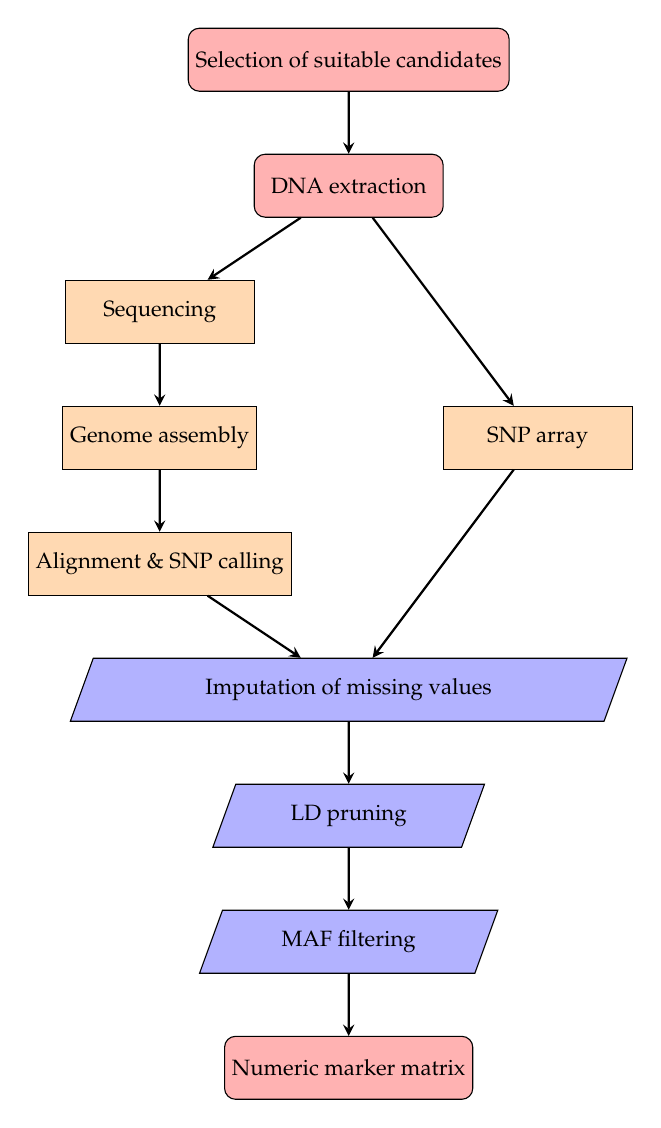
\begin{tikzpicture}[node distance=2cm, scale=0.8, transform shape]
      \node (start0) [startstop] {Selection of suitable candidates};
      \node (start) [startstop,below of=start0] {DNA extraction};
      \draw [arrow] (start0) -- (start);
      \node (seq) [process, below of=start, xshift=-3cm] {Sequencing} ;
      \draw [arrow] (start) -- (seq);
      \node (SNP) [process, below of=start, xshift=3cm, yshift=-2cm] {SNP array} ;
      \draw [arrow] (start) -- (SNP);
      \node (ga) [process, below of=seq] {Genome assembly} ;
      \draw [arrow] (seq) -- (ga);
      \node (snpca) [process, below of=ga] {Alignment \& SNP calling} ;
      \draw [arrow] (ga) -- (snpca);
      \node (imp) [io, below of=snpca, xshift=3cm] {Imputation of missing values};
      \draw [arrow] (snpca) -- (imp) ;
      \draw [arrow] (SNP) -- (imp) ;
      \node (LD) [io, below of=imp] {LD pruning} ;
      \draw [arrow] (imp) -- (LD) ;
      \node (MAF) [io, below of=LD] {MAF filtering} ;
      \draw [arrow] (LD) -- (MAF) ;
      \node (bm) [startstop, below of=MAF] {Numeric marker matrix} ;
      \draw [arrow] (MAF) -- (bm) ;
    \end{tikzpicture}
    \caption[Schematic process of genotyping for quantitative genetics]{Schematic process of genotyping for quantitative genetics analyses with its crucial steps} \label{fig:quan_flow1}
  \end{center}     
\end{figure}

Chapter \ref{Chapter1} will focus on the first parts of figure \ref{fig:quan_flow1}, the
assembly of genomes exemplified with plastid genomes and will elucidate some of the major
obstacles presented, when starting with raw DNA reads and going to data, which is suitable
for quantitative methods like GWAS and genomic selection. Section \ref{Chapter2} will
introduce a novel tool to perform large-scale GWAS using modern software and computing
resources. \\
Chapter \ref{Chapter3} will give in depth introductions to machine learning and the
complex architecture of quantitative traits and bring them in the context of plant
breeding and how those techniques can be used to continue improving plant germplasms for
modern agriculture. Genomic selection is a process during which plants are not only
selected and assessed based on their bare phenotypic appearances or pedigree relatedness
to other individuals but also based on their genomic features \cite{hayes2001}. \\
In the final chapter figure \ref{fig:quan_flow1} will be recapitulated and the main
obstacles in the process will be thoroughly decomposed and explained how this study aids
in providing solutions for some of them. 





%%% Local Variables:
%%% mode: latex
%%% TeX-master: "../main"
%%% End:

% Chapter 1



\chapter{Benchmarking of Chloroplast Genome Assembly tools } % Main chapter title

\label{Chapter1} % For referencing the chapter elsewhere, use \ref{Chapter1}
This chapter orientates on \cite{freudenthal2019landscape} only the chapters from the publication which the author majorly contributed to are included. 

%----------------------------------------------------------------------------------------

% Define some commands to keep the formatting separated from the content 
\newcommand{\keyword}[1]{\textbf{#1}}
\newcommand{\tabhead}[1]{\textbf{#1}}
\newcommand{\code}[1]{\texttt{#1}}
\newcommand{\file}[1]{\texttt{\bfseries#1}}
\newcommand{\option}[1]{\texttt{\itshape#1}}

%----------------------------------------------------------------------------------------

\section{Introduction}

Circular DNA of a size between 120 kBP to 160 kBP \cite{palmer_1985}.  First chloroplast sequenced as early
as 1986 \textit{Marchantia polymorpha} and \textit{Nico} \cite{ohyama_chloroplast_1986}; \cite{shinozaki_complete_1986}.
Review  genome structure \cite{green_chloroplast_2011}; \cite{wicke_evolution_2011}.
Chloroplast genomes widely used in evolutionary studies \cite{martin_evolutionary_2002}; \cite{xiao-ming_inferring_2017}.
Chloroplast genomes are small through endosymbiotic gene transfer \cite{martin_evolutionary_2002}; \cite{deiner_environmental_2017}. Up to 14 \% of the the core genome of \textit{Arabidopsis thaliana} is made up of genes previously from the chloroplast (fancy citation), while 100-120 genes remain on the chloroplast \cite{wicke_evolution_2011}.
However chloroplast between plant species show large variety e.g. parasitic plants.
Chloroplast genomes are much smaller than core genomes e.g \textit{A. thaliana} ca. 125 MBP. Highly conserved high gene content, therefore changes are more likely to be functional.
Single chloroplast contain up to hundreds of copies of its genome \cite{kumar_2014}; \cite{bendich_1987}, and photosynthetic activate cells contain multiple chloroplasts, therefore the copy number of chloroplast genomes is much higher than number of core genomes per cell.
Structurally chloroplast genomes consist of two inverted repeats (IR) - $IR_A$ and $IR_B$ -  ranging from 10 kbp to 76 kB the divide the chloroplast genome into two distinct regions the large single copy (LSC) and the small single copy (SSC) as shown in \ref{fig:cpast_genome} \cite{palmer_1985}. Taking into account that the majority of assembly tools has been designed to assemble linear core genomes, the structure of chloroplast genomes is a major obstacle when wanting to assemble those genomes with modern short read technologies, especially solving and aligning the IR \cite{Wang2018}.

\begin{figure}[H]
\centering
\includegraphics[height=.55\textheight, width=.95\textwidth]{Figures/cpast}
\decoRule
\caption[Structure of a chloroplast genome]{Structure of the chloroplast genome of \textit{A. thaliana} with SSC-Region and LSC-Region. Length of the genome and its parts in kbp. Graphic from \cite{olejniczak2016chloroplasts}
\label{fig:cpast_genome}
\end{figure}




%----------------------------------------------------------------------------------------
\section{Material and Methods}
\subsection{Methods}
\subsection{Tools}
\subsection{Evaluation}
\subsubsection{Quantitative}
\begin{equation}
  score = \frac{1}{4} \cdot \left( cov_{ref} +  cov_{qry} + min\left\{ \frac{cov_{qry}}{cov_{ref}}, \frac{cov_{ref}}{cov_{qry}}\right\} + \frac{1}{n_{contiguous} }\right) \cdot 100 
\label{eqn:score_ass}
\end{equation}

\subsubsection{Qualitative}
\subsubsection{Consistency}


\subsection{Data}
\subsubsection{Simulated}
\subsubsection{Real data set}
\subsubsection{Novel data set}


\section{Results}
\subsection{Qualitative}

\subsection{Quantitative}
\subsubsection{Simulated data}
\begin{figure}[H]
\centering
\includegraphics[height=.45\textheight, width=.95\textwidth]{Figures/sim_tiles}
\decoRule
\caption[Score of assemblies of simulated data sets]{Results of assemblies executed with simulated data sets.}
\label{fig:sim_tiles}
\end{figure}



\begin{table}[h!]
\caption{\textbf{Scores of assemblies of simulated data}}
\label{tab:scores_simulated}
\centering
\begin{tabular}{rlrrrrrrr}
  \hline
  & data set & CAP & CE & Fast-Plast & GetOrganelle & IOGA & NOVOPlasty & org.ASM \\ 
  \hline
  1 & sim\_150bp.0-1 & 79.10 & 100.00 & 99.48 & 100.00 &  & 91.52 & 100.00 \\ 
  2 & sim\_150bp.0-1.2M & 79.10 & 100.00 & 99.72 & 100.00 & 79.10 & 91.52 & 91.50 \\ 
  3 & sim\_150bp.1-10 &  & 56.44 & 100.00 & 76.98 &  & 91.52 & 78.00 \\ 
  4 & sim\_150bp.1-10.2M &  &  & 99.97 & 100.00 &  & 91.52 & 82.72 \\ 
  5 & sim\_150bp.1-100 & 75.72 & 100.00 & 99.48 & 100.00 & 66.09 & 91.52 & 91.50 \\ 
  6 & sim\_150bp.1-100.2M &  & 100.00 & 99.47 & 100.00 &  & 100.00 & 100.00 \\ 
  7 & sim\_150bp.1-1000 & 79.10 &  & 99.72 & 100.00 &  & 91.52 & 100.00 \\ 
  8 & sim\_150bp.1-1000.2M & 79.10 & 100.00 & 99.72 & 100.00 &  & 91.52 & 100.00 \\ 
  9 & sim\_250bp.0-1 & 79.10 & 100.00 & 93.82 & 100.00 &  & 91.52 & 91.50 \\ 
  10 & sim\_250bp.0-1.2M & 79.10 & 100.00 & 93.83 & 100.00 &  & 91.52 & 91.50 \\ 
  11 & sim\_250bp.1-10 &  & 54.98 & 68.45 & 78.89 & 52.71 & 91.52 & 40.20 \\ 
  12 & sim\_250bp.1-10.2M &  &  & 93.00 & 100.00 & 52.67 & 87.40 & 40.20 \\ 
  13 & sim\_250bp.1-100 & 72.81 & 100.00 & 93.82 & 100.00 &  & 87.40 & 100.00 \\ 
  14 & sim\_250bp.1-100.2M &  & 100.00 & 93.83 & 100.00 &  & 87.40 & 100.00 \\ 
  15 & sim\_250bp.1-1000 & 79.10 & 21.30 & 93.83 & 100.00 & 76.96 & 91.52 & 91.50 \\ 
  16 & sim\_250bp.1-1000.2M & 79.10 & 100.00 & 93.83 & 100.00 & 67.55 & 87.40 & 100.00 \\
  \hline
\end{tabular}
\end{table}




\subsubsection{Real data sets}
\begin{table}[h!]
\caption{\textbf{Mean scores of chloroplast genome assemblers}}
\label{tab:scores_real}
\centering
\begin{tabular}{rlrrrr}
  \hline
 & assembler & Median & IQR & N\_perfect & N\_tot \\ 
  \hline
1 & CAP & 45.25 & 50.19 &   0 & 369 \\ 
  2 & CE & 56.55 & 71.50 &  14 & 369 \\ 
  3 & Fast-Plast & 92.80 & 23.59 & 113 & 369 \\ 
  4 & GetOrganelle & 99.83 & 20.94 & 210 & 360 \\ 
  5 & IOGA & 71.10 & 11.21 &  0 & 338 \\ 
  6 & NOVOPlasty & 75.95 & 48.69 &  58 & 369 \\ 
  7 & org.ASM & 67.35 & 91.69 &  46 & 348 \\ 
   \hline
\end{tabular}
\end{table}





\begin{figure}[H]
\centering
\includegraphics[height=.45\textheight, width=.95\textwidth]{Figures/swarm}
\decoRule
\caption[Scores of assemblies from real data sets]{Box and swarm plots depict the results from the scoring shown in \ref{eqn:score_ass}}
\label{fig:swarm}
\end{figure}




\subsubsection{Consistency}

\subsubsection{Real data sets}
\begin{figure}[H]
\centering
\includegraphics[height=.45\textheight, width=.95\textwidth]{Figures/repro}
\decoRule
\caption[Comparison between two runs with the same assembler for consistency testing ]{Swarm plots depict the results from the scoring shown in \ref{eqn:score_ass} for two independent runs for each assembler on each of the data sets}
\label{fig:consisplot}
\end{figure}


\subsubsection{Novel}


\begin{figure}[H]
\centering
\includegraphics[height=.45\textheight, width=.95\textwidth]{Figures/upset_novel}
\decoRule
\caption[Upset plot comparing the success rates for novel data sets]{nls}
\label{fig:upset_novel}
\end{figure}

\section{Discussion}

\begin{figure}[H]
\centering
\includegraphics[height=.45\textheight, width=.95\textwidth]{Figures/upset}
\decoRule
\caption[Upset plot comparing the success rates of of all assemblers]{Upset plot showing the intersections of success rates between assemblers. A successful assembly was defined with a score > 99 according to equation \ref{eqn:score_ass}}
\label{fig:upset}
\end{figure}



%% Chapter 1

\chapter{Understanding the hapoltype structure of Arabidopisis thaliana } % Main chapter title

\label{Chapter1} % For referencing the chapter elsewhere, use \ref{Chapter1} 

%----------------------------------------------------------------------------------------



\section{Introduction}

\section{Haplotyping of A. thaliana}

\section{Results}

\begin{figure}[th]
\centering
\includegraphics[height=.55\textheight, width=1.1\textwidth]{Figures/chr1_hap}
\decoRule
\caption[Haplotype strutcture of chromosome 1 of \textit{A. thaliana}]{The number of segregating haplotypes with a polymorphism in at least one position over a stretch of 1 kBP. }
\label{fig:chr1}
\end{figure}



\begin{figure}[th]
\centering
\includegraphics[height=.55\textheight, width=1.1\textwidth]{Figures/chr2_hap}
\decoRule
\caption[Haplotype strutcture of chromosome 2 of \textit{A. thaliana}]{Number of segregating haplotypes with a polymorphism in at least one position over a stretch of 1 kBP. }
\label{fig:chr2}
\end{figure}


\begin{figure}[th]
\centering
\includegraphics[height=.55\textheight, width=1.1\textwidth]{Figures/chr3_hap}
\decoRule
\caption[Haplotype strutcture of chromosome 3 of \textit{A. thaliana}]{Number of segregating haplotypes with a polymorphism in at least one position over a stretch of 1 kBP. }
\label{fig:chr3}
\end{figure}


\begin{figure}[th]
\centering
\includegraphics[height=.55\textheight, width=1.1\textwidth]{Figures/chr4_hap}
\decoRule
\caption[Haplotype strutcture of chromosome 4 of \textit{A. thaliana}]{Number of segregating haplotypes with a polymorphism in at least one position over a stretch of 1 kBP. }
\label{fig:chr4}
\end{figure}


\begin{figure}[th]
\centering
\includegraphics[height=.55\textheight, width=1.1\textwidth]{Figures/chr5_hap}
\decoRule
\caption[Haplotype strutcture of chromosome 5 of \textit{A. thaliana}]{Number of segregating haplotypes with a polymorphism in at least one position over a stretch of 1 kBP. }
\label{fig:chr5}
\end{figure}





\section{Disucssion}


\begin{figure}[th]
\centering
\includegraphics[height=.55\textheight, width=1.1\textwidth]{Figures/plot_NAs_AT}
\decoRule
\caption[blabl]{Number of segregating haplotypes with a polymorphism in at least one position over a stretch of 1 kBP. }
\label{fig:chr_bla}
\end{figure}




 
% -*- TeX-master: "main.tex" -*-
% Chapter 1

\chapter{GWAS-Flow a gpu-accelerated software for large-scale genome-wide association studies}

\label{Chapter3} % For referencing the chapter elsewhere, use \ref{Chapter1} 

%----------------------------------------------------------------------------------------

The following chapter has been published in a similar version on the bio$\chi$iv preprint
server \cite{Freudenthal_2019} and has been submitted for publication. The experiments and
the software were designed and conducted by the author. The manuscript has been prepared
by the author, with minor corrections from Prof. Arthur Korte \& Prof. Dominik Grimm. All
authors approved of the final manuscript.


\section{Introduction}
Genome-wide association studies, pioneered in human genetics \cite{Hirschhorn2005} have
become the predominant method to detect associations between phenotypes and the genetic
variations present in a population, in the last decade. Understanding the genetic
architecture of traits and mapping the underlying genomic polymorphisms is of paramount
importance for successful breeding, both in plants and animals, as well as for studying
the genetic risk factors of diseases. Over the last decades the costs for genotyping have
been reduced dramatically. Early GWAS consisted of a few hundred individuals, which have
been phenotyped and genotyped on a couple of hundreds to thousands of genomic
markers. Nowadays marker densities for many species easily exceed millions of genomic
polymorphisms. Albeit commonly SNPs are used for association studies, standard GWAS models
are flexible to handle different genomic features as input. \\
The \textit{Arabidopsis} 1001 genomes project features for example 1135 sequenced
\textit{Arabidopsis thaliana} accessions with over 10 million genomic markers that
segregate in the population \cite{1001genome}. Other genome projects also yielded large
amounts of genomic data for a substantial amount of individuals, as exemplified in the
1000 genomes project for humans \cite{1000genome}, the 2000 yeast genomes project or the
3000 rice genomes project \cite{3000genome}. Thus, there is an increasing demand for GWAS
models that can analyze these data in a reasonable time frame.\\
One critical step of GWAS is to determine the threshold at which an association is termed
significant. Classically the conservative Bonferroni threshold is used, which accounts for
the number of statistical tests that are performed, while many recent studies try to set
significance thresholds that are based on the false-discovery rate (FDR)
\cite{Storey9440}. An alternative approach to determine permutation-based thresholds
\cite{che2014adaptive}. Permutation-based thresholds estimate the significance by
shuffling phenotypes and genotypes before each GWAS run, thus any signal left in the data
should not have a genetic cause, but might represent model mis-specifications or uneven
phenotypic distributions. Typically this process is repeated hundreds to thousands of
times and will lead to a distinct threshold for each phenotype analyzed
\cite{togninalli2017aragwas}. The computational demand of permutation-based thresholds is
immense, as per analysis not one, but at least hundreds of GWAS need to be performed. Here
the main limitation is the pure computational demand. Thus, faster GWAS models could
easily make the estimation of permutation-based thresholds the default choice.

\section{Methods}

\subsubsection{GWAS Model}
The GWAS model used for \texttt{GWAS-Flow} is based on a fast approximation of the
linear-mixed-model described in \cite{kang2010variance,Zhang2010}, which estimates the
variance components $\sigma$\textsubscript{g} and $\sigma$\textsubscript{e} only once in a
null model that includes the genetic relationship matrix but no distinct genetic
markers. These components are thereafter used for the tests of each specific marker. Here,
the underlying assumption is that the ratio of these components stays constant, even if
distinct genetic markers are included into the GWAS model. This holds true for nearly all
markers and only markers, which posses a big effect will alter this ratio slightly, where
now $\sigma$\textsubscript{g} would become smaller compared to the null model. Thus, the
p-values calculated by the approximation might be a little higher (less significant) for
strongly associated markers.

\subsubsection{The GWAS-Flow Software}
The \texttt{GWAS-Flow} software was designed to provide a fast and robust GWAS
implementation that can easily handle large data and allows to perform permutations in a
reasonable time frame. Traditional GWAS implementations that are implemented using Python
\cite{van1995python} or R \cite{R} cannot always meet these demands. We tried to overcome
those limitations by using TensorFlow, a multi-language machine learning framework
published and developed by Google \cite{tensorflow2015-whitepaper}. GWAS calculations are
composed of a series of matrix computations that can be highly parallelized and easily
integrated into the architecture provided by TensorFlow. Our implementation allows both
the classical parallelization of code on multiple processors (CPUs) and the use of
graphical processing units (GPUs).\\
\texttt{GWAS-Flow} is written using the Python TensorFlow API. Data import is done with
\textit{pandas} \cite{mckinney-proc-scipy-2010} and/or \textit{HDF5} for Python
\cite{hdf5_2014}. Preprocessing of the data (e.g filtering by minor Allele count (MAC)) is
performed with \textit{numpy} \cite{oliphant2006guide}. Variance components for residual
and genomic effects are estimated with a function slightly altered from the Python package
\textit{limix} \cite{Lippert003905}. The GWAS model is based on the following linear mixed
model that takes into account the effect of every marker with respect to the kinship:

\begin{equation}
Y = \beta_{0} + X_i\beta_i + u + \epsilon, u \sim N(0,\sigma_gK), \epsilon \sim N(0,\sigma_e I )
\label{eqn:LMM GWAS}
\end{equation}

\noindent
From this LMM the residual sum of squares for marker $i$ are calculated as described in
\ref{eqn:RSS_GWAS}

\begin{equation}
RSS_{i} = \sum{Y - (X_{i}\beta_{0}  + I_{i}\beta_{1})}
\label{eqn:RSS_GWAS}
\end{equation}

\noindent
The residuals are used to calculate a p-value for each marker according to an overall
F-test, which compares the model including a distinct genetic effect to a model without
this genetic effect:

\begin{equation}
 F = \frac{RSS_{env} - R1_{full} }{\frac{R1_{full}}{n-3}}
 \label{F_test}
\end{equation}

\noindent
Apart from the p-values that derive from the F-distribution, \texttt{GWAS-Flow} also
reports summary statistics, such as the estimated effect size ($\beta_i$) and its standard
error for each marker.

\subsubsection{Calculation of permutation-based thresholds for GWAS}

To calculate a permutation-based threshold essentially \textit{n} repetitions (\textit{n}
$\geq$ 100) are computed of the GWAS on the same data with the sole difference that before
each GWAS phenotypic values are randomized. Thus any correlation between the phenotype and
the genotype will be broken and indeed for over 90\% of these analyses the estimated
pseudo-heritability is close to zero. On the other hand, the phenotypic distribution will
stay unaltered by this randomization. Hence any remaining signal in the GWAS has to be of
a non-genetic origin and could be caused by e.g. model mis-specifications. Now the lowest
p-value (after filtering for the desired minor allele count) is taken for each permutation
and the 5\% lowest value is set as the permutation-based threshold for the GWAS.

\subsubsection{Benchmarking}

For benchmarking of \texttt{GWAS-Flow} data from the \textit{Arabidopsis} 1001 Genomes
Project \cite{1001genome} was used. The genomic data used were subsets of the full data
set containing between 10,000 and 100,000 markers. Subsets that exceed 100,000 markers
were not included because there is a linear relationship between the number of markers and
the computational time demanded, as all markers are tested independently. Phenotypic data
for flowering time at ten degrees (FT10) for \textit{A. thaliana} was used, downloaded
from the AraPheno database \cite{seren2016arapheno}. Down- and up-sampled sets were
generated to obtain phenotypes for sets between 100 and 5000 accessions. For each set of
phenotypes and markers 10 permutations were run to assess the computational time
necessary.\\
All analyses have been performed with a custom R script that has been used previously
\cite{togninalli2017aragwas}, \texttt{GWAS-Flow} using either a CPU or a GPU architecture
and \textit{GEMMA} \cite{Zhou2012}. \textit{GEMMA} is a fast and efficient implementation
of the mixed model that is broadly used to perform GWAS. All calculations were run on the
same machine using 16 i9 virtual CPUs. The GPU version ran on an NVIDIA Tesla P100 graphic
card. Additionally to the analyses of the simulated data, the times required by
\textit{GEMMA} and both \texttt{GWAS-Flow} implementations for $>$ 200 different real
data sets from \textit{A. thaliana} were compared, which also have been downloaded from the
AraPheno database \cite{seren2016arapheno} and have been analyzed with the available fully
imputed genomic data set of ca. 10 million markers, filtered for a minor allele count
greater five.

\section{Results}

The two main factors influencing the computational time for GWAS are the number of markers
incorporated in such an analysis and the number of different accessions, while the latter
has an approximate quadratic effect in classical GWAS implementations
\cite{Zhou2012}. Figure \ref{fig:time_accessions} shows the time demand as a function of
the number of accessions used in the analysis with 10,000 markers. Exponential increases
in the time demand are clearly visible for the custom R implementation, as well as for the
CPU-based \texttt{GWAS-Flow} implementation and \textit{GEMMA}. The \texttt{GWAS-Flow}
implementations and \textit{GEMMA} clearly outperform the R implementation in general.
For a smaller number of accessions \texttt{GWAS-Flow} is slightly faster then
\textit{GEMMA}.\\
For the GPU-based implementation the increase in run-time with larger sample sizes is much
less pronounced. While for small ($< 1,000$ individuals) data there is no benefit
compared to running \texttt{GWAS-Flow} on CPUs or running \textit{GEMMA}, the GPU-version
clearly outperforms the other implementations if the number of accessions increases.

\begin{figure}[H]
\centering
\includegraphics[height=.55\textheight, width=1.1\textwidth]{Figures/comp_time_gwas}
\decoRule
\caption[Computations time vs accessions]{Computational time as a function of the number
  of accessions with 10000 markers each.}
\label{fig:time_accessions}
\end{figure}

Figure \ref{fig:time_marker} shows the computational time in relation to the number of
markers with a fixed population of 2000 accessions for the two different
\texttt{GWAS-Flow} implementations. Here, a linear relationship is visible in both
cases.\\
To show the performance of \texttt{GWAS-Flow} not only for simulated data, both
implementations were also run on more than 200 different real data sets of
\textit{A. thaliana}. Figure \ref{fig:real_data_gwas} shows the computational time demands for all analyses
comparing both \texttt{GWAS-Flow} implementations to \textit{GEMMA}. Here, the CPU-based
\texttt{GWAS-Flow} performs comparable to \textit{GEMMA}, while the GPU-based
implementation outperforms both if the number of accessions is above 500. Importantly all
obtained GWAS results (p-values, beta estimates and standard errors of the beta estimates)
are nearly (apart from some mathematical inaccuracies) identical between the three
different implementations.

\begin{figure}[H]
\centering
\includegraphics[height=.55\textheight, width=1.1\textwidth]{Figures/time_markers_gwas}
\decoRule
\caption[Computation time vs number of markers]{Computational time as a function of the number of genetic markers with constantly 2000 accessions for both \texttt{GWAS-Flow} versions}
\label{fig:time_marker}
\end{figure}

\section{Discussion}

To cope with the increasing computational demand in analyzing large GWAS data sets, recent
developments of computational architecture and software were utilized to develop
\texttt{GWAS-Flow}. With \texttt{GWAS-Flow} both a CPU- and a GPU-based version of the
classical linear mixed model, commonly used for GWAS, is provided. Both implementations
outperform custom R scripts on simulated and real data. While the CPU-based version
performs nearly identical compared to \textit{GEMMA}, a commonly used GWAS implementation,
the GPU-based implementation outperforms both, if the number of individuals, which have
been phenotyped, increases. For analyzing big data, here the main limitation would be the
RAM of the GPU, but as the individual test for each marker is
independent, this can be easily overcome programmatically. \\
The presented \texttt{GWAS-Flow} implementations are markedly faster compared to custom
GWAS scripts and even outperform efficient fast implementations like \textit{GEMMA} in
terms of speed. This readily enables the use of permutation-based thresholds, as with
\texttt{GWAS-Flow} hundred permutations can be performed in a reasonable time frame even
for big data. Thus, it is possible for each analyzed phenotype to create a specific,
permutation-based threshold that might present a more realistic scenario. Importantly the
permutation-based threshold can be easily adjusted to different minor allele counts,
generating different significance thresholds depending on the allele count. This could
help to distinguish false and true associations even for rare alleles.\\
\texttt{GWAS-Flow} is a versatile and fast software package and currently is and will
remain under active development to make the software more versatile. This will e.g. to
include the compatibility with TensorFlow v2.0.0 and to enable data input formats, such as
PLINK \cite{purcell2007plink}. The whole framework is flexible, so it is easy to include
predefined co-factors e.g to enable multi-locus models \cite{segura2012efficient} or
account for multi-variate models like the multi-trait mixed model
\cite{korte2012mixed}. \\
Standard GWAS are good in detecting additive effects with comparably large effect sizes,
but lack the ability to detect epistatic interactions and their influence on complex
traits \cite{mckinney2012six}; \cite{korte2013advantages}. To catch the effects of these
gene-by-gene or SNP-by-SNP interactions, a variety of genome-wide association interaction
studies (GWAIS) have been developed, thoroughly reviewed in \cite{ritchie2018GWAIS}. Here,
\texttt{GWAS-Flow} might provide a tool that enables to test the full pairwise interaction
matrix of all SNPs. Although this would be a statistic nightmare, it now would be
computationally feasible.


\begin{figure}[H]
 \centering \includegraphics[height=.6\textheight, width=1.1\textwidth]{Figures/gwas_real_data} \decoRule
 \caption[Computational time of GWA Analyses on real \textit{A. thaliana} data
 sets]{Comparison of the computational time for the analyses of $>$ 200 phenotypes from
   \textit{Arabidopsis thaliana} as a function of the number of accessions for
   \textit{GEMMA} and the CPU- and GPU-based version of \texttt{GWAS-Flow}. GWAS was
   performed with a fully imputed genotype matrix containing 10.7 M markers and a minor
   allele filter of MAC $>5$}
\label{fig:real_data_gwas}
\end{figure}





%%% Local Variables:
%%% mode: latex
%%% TeX-master: "../main"
%%% End:


\chapter{Genomic prediction of phenotypic values of quantitative traits using Artificial neural networks}

\label{Chapter3} % For referencing the chapter elsewhere, use \ref{Chapter1} 

%----------------------------------------------------------------------------------------



\section{Introduction}
\subsection{A brief history of machine learning }

While machine learning, neural networks, deep learning became essential tools for many applications in more recent years,
their mathematical principals date back to the early 1950s and 1960s. Figure \ref{fig:perceptron} schematically  show the
basic perceptron model as proposed by Rosenblatt, which was designed to mimic the information flow in biological nervous systems
\cite{rosenblatt1961}

\begin{figure}[th]
\centering
\includegraphics[height=.25\textheight, width=.5\textwidth]{Figures/perceptron.png}
\decoRule
\caption[Basic perceptron model]{Basic perceptron model as proposed by Rosenblatt}
\label{fig:perceptron}
\end{figure}

This basic perceptron, which contrary to perceptrons used nowadays does not have an activation function, takes n binary
inputs $x_1 , x_2 .... x_n$ and produces a single, likewise binary, output $y$ after being processed by the perceptron or neuron.
To achieve this Rosenblatt introduced the concept of weights which indicated a certain relative importance to the outcome of the
output. $w_1 , w_2 ... w_n$. The output $y$ is determined by the weighted sum of the weights and biases $\sum_i w_ix_i $. If a certain
threshold value is met  the neuron is either activated and outputs 1 or not and outputs 0. This is algebraically represented in
\ref{eqn:weights}
\begin{subequations}
  \begin{align}
    0  = \mbox{if } \sum_i^n w_j x_i - \theta \leq 0 \\
    1 =  \mbox{if } \sum_i^n w_i x_i - \theta > 0
  \end{align}
  \label{eqn:weights}
\end{subequations}

Next to the weights $w_n$ and the inputs $x_n$ a third term $\theta$ is introduced in equation \ref{eqn:weights} which represents
the activation threshold in per definition is negative. A single perceptron is a linear classifier and can only be trained on
linearly separable functions and can used as shown by \cite{rosenblatt1961} to solve simple logical operations as AND, OR and not.
The simple perceptron fails, due to non-linearity, to perform XOR operations as shown by \cite{marvin1969}. This discovery let to
a near stillstance in the research of artificial neural networks in the 1970s.



\subsection{On the nature of quantitative traits}
According to the omnigenic model which is an extension of the polygenic model proposed by \cite{boyle2017expanded} and
thoroughly reviewed in \cite{timpson2018} all traits or phenotypic values are influenced
by a great number or all genes in the genome. Therefore resulting in traits following certain gradual statistical distributions
instead of being binned in classes or even binary. Intuitively this might be contradicting with the foundation of modern Genetics -
Mendel's three laws. That where derived from observations with where mainly influenced by one locus. But staying with one of
Mendel's examples the round or wrinkled surfaces of  peas \textit{Pisum sativum}, an assessment of a couple of thousands peas, would
most likely inevitably
lead to the conclusion that form the ``roundest'' to the ``wrinkliest'' pea any gradual step between those is possible and observable.
Mendel's third law of independent segregation also only holds true under certain assumptions. The most simplest one being that the traits
under investigation have to be located on different linkage groups. Otherwise for the 7 traits used in Mendel's initial studies would not have
segregated independently. The odds of 7 randomly selected traits being on 7 different linkage groups are rather small, especially taking
into account, that the genome of the \textit{P. sativum} consists of only 7 chromosomes itself \cite{kalo2004}. Mendel probably new about
traits not following its own law's,
as well as being aware of the quantitative nature of traits such as the constitution of surfaces of peas or the color of petals. But being the
pioneer of a then rather unexplored field of science, some of which big questions we fail to satisfactory answer today, he did not have the
resources or the knowledge to explain behavior's not ``mendeling'', that were only able to be deciphered in later decades and centuries
based on his ground-breaking work.  \\
Initially thought to be contradicting to Mendel's ideas Darwin proposed the concept's of evolution due to natural selection which also
introduce the idea of traits following a gradual distribution \cite{darwin1859}. This contrast led to a long lasting debate in the
scientific community in the early 1900s, between the Mendelians and the biometricians who believed in the quantitative nature of continuous
traits. This conflict has eventually been solved by Fisher's fundamental work published in 1918 \cite{fisher1919xv}. His theroies combined the
then in all fields of science popular research of distributions with genomics. He he mathematically proved that traits influenced by many
genes, with randomly-sampled alleles follow a continous normal distrubition in a population. While this combined the indeas of Mendel and the
biometricans it opened an other long debated queston of effect size and the overall architecture of complex traits. While in the theory of
monogenic traits the effect size of the single gene on the trait is 1 or 100 \% with an increasing number of genes influecning a complex
traits the \textit{per sè} contribution of single gene has to decrease with an increasing number of loci determining the value a given
trait. In the 1990s it has been thought, that complex traits are predominantly controlled from few genes with a large to medium effect size,
while others had a minimal influence \cite{zhang2018esti}. \\
With the upcomming popularity of GWAS as the favored method to decipher genetic archtitectures of traits, or having pioneered in human
genetics in became clear that the majority of the effect sizes are tiny < 1 \% while there are very few loci which have a moderate
effect on the phenotypic variance of a population with around 10 \% or less \cite{korte2013advantages}, \cite{stringer2011}.
This nature of quantitative traits present greate challenges to animal \cite{goddard2009} and plant breeding \cite{wurschum2012},
in further improving crop or livestock performances, as well complicating the decomposition of genomic causes for diseases like shiozphrania
or autism in human medicine \cite{de2014}, \cite{purcell2014}. \\
While the complex nature of the architecture of quantitave traits provide enough challanges as is, all traits will also be influenced
by the evironment from which an induvidual originates.
Therefore the distribution of trait valaues in a given population can be expressed as the addition of the variances of its genetic and the
environemtnal effects \ref{eqn:PGE}.

\begin{equation}
  \sigma_{P} = \sigma_{G} + \sigma_{E}
  \label{eqn:PGE}
\end{equation}

The genomic and the evironmental effects not only influnce the phenotypic variance directly, but the environment also has an influnce
on gene expression methylation of DNA bases etc. and therefore the equation \ref{eqn:PGE} needs to be extend by the variance of the gene-
environment interactions $\sigma_{GxE}$  \ref{eqn:PGEGE} , \cite{lynch1998}, \cite{walsh2018}.
                                                               
\begin{equation}
  \sigma_{P} = \sigma_{G} + \sigma_{E} + \sigma_{GxE}
  \label{eqn:PGGE}
\end{equation}


Equation \ref{eqn:PGGE} shows the decomposition of the phenotypic variance, to thoroughly understand complex genetic archiectures of traits
the genetic variance needs to be decomposed further in its additve, dominance and epistatic components \ref{eqn:GAD}

\begin{equation}
  \sigma_{G} = \sigma_{A} + \sigma_{D} + \sigma_{I}
  \label{eqn:GAD}
\end{equation}

The addivte effects are caused by single, for this model mostly homozygous, loci while the variance caused by dominance effcts, is caused by
heterozygous loci and their resulting interactions being full-, over- , co- or underdominant. And lastely the interaction effects  that are a
result of two or more genes only having an impact if the involved genes cooccur in a certain state. The resulting variance is commonly known
as gene-gene interactions and/or epistasis \cite{falconer1996}. \\
Since possible interactions in a genome can happen between additve or dominant or a combinaton of those loci. The variance due to interaction
effects $\sigma_{I}$ can be further dissembled in the variance resulting from additive-addtive $\sigma_{AA}$ domiant-dominant $\sigma{DD}$ and
additive-dominant $sigma{AD}$ terms as represented in equation \ref{eqn:IAA}.


\begin{equation}
  \sigma_{I} = \sigma_{AxA} + \sigma_{DxD} + \sigma_{AxD}
  \label{eqn:IAA}
\end{equation}

Knowledge of the variace components involved in the expression of a trait in population, lead up to the estimation of the total influnce
of all genetic variances and the environmental variance one the phentypic distrubition. This concept if called heritabilty.
The heritabilty of a trait $h^2$ accounts for the proportion of the pheotyping variace controlled by the total phenotypic variance.




\begin{equation}
  h^2 = \frac{\sigma_{G}}{\sigma_{P}}
  \label{eqn:h2G}
\end{equation}


\begin{equation}
  h^2 = \frac{\sigma_{A}}{\sigma_{P}}
  \label{eqn:h2a}
\end{equation}







\subsection{Genomic selection using artificial neural networks }
Genomic selection (GS) has been successfully applied in animal \cite{gianola2015one}, \cite{hayes2010genome}
and plant breeding \cite{crossa2010}, \cite{desta2014genomic}, \cite{heffner2010plant}, \cite{crossa2017genomic}
as well as in medical applications, since it was first reported  \cite{hayes2001}. Since then the repertoire of
methods for predicting phenotypic values has increased rapidly e.g.\cite{dlc2009}, \cite{habier2011}, \cite{gianola2013} ,
\cite{crossa2017}. The most commonly applied methods include GULP and a set of related algorithms known as the bayesian alphabet
\cite{gianola2009}. 
Genomic prediction in general has repeatedly been shown to outperform pedigree-based methods \cite{crossa2010},
\cite{albrecht2011} and is nowadays used in many plant and animal breeding schemes. 
It has also been shown that using whole-genome information is superior to using only feature-selected markers
with known QTLs for a given trait \cite{bernardo2007}, \cite{heffner2011} in some cases. A more recent study
\cite{azodi2019} compared 11 different genomic prediction algorithms with a variety of data sets and found
contradicting results, indicating that feature selection can be usefull in some cases the when the whole
genome regression is performed by neural nets 
While every new method is a valuable addition to the tool-kits for genomic selection, some fundamental
problems remain unsolved, of which the n>>p problematic stands out. Usually in genomic selection settings
the size of the training population (TRN) with n phenotypes is substantially smaller than the number of
markers (p) \cite{fan2014challenges}. Making the number of features immensely large,  even when SNP-SNP
interactions are not considered.  Furthermore each marker is treated as an independent observation
neglecting collinearity and linkage disequilibrium (LD). 
Further difficulties arise through non-additive, epistatic and dominance marker effects. The main problem
with epistasis issue quantitative genetics is the almost infinite amount of different marker combinations,
that cannot be represented within the size of TRN in the thousands, the same problems arises for example
in GWA studies \cite{korte2013advantages}. With already large p the number of possible additive SNP-SNP interactions
potentiates to $p^{(p-1)}$. Methods that attempt to overcome those issues are EG-BLUP, using an enhanced
epistatic kinship matrix and reproducing kernel Hilbert space regression (RKHS) \cite{jiang2015}, \cite{martini2017genomic}.

In the past 10 years, due to increasing availability of high performance computational hardware with decreasing
costs and parallel development of free easy-to-use software, most prominent being googles library TensorFlow
\cite{TF2016} and Keras \cite{keras2015}, machine learning (ML) has experienced a renaissance.
ML is a set of methods and algorithms used widely for regression and classification problems. popular
among those are e.g. support vector machines, multi-layer perceptrons (MLP) and convolutional neural
networks. The machine learning mimics the architecture of neural networks and are therefore commonly
referred to as artificial neural networks (ANN). Those algorithms have widely been applied in many
biological fields \cite{min2017deep} , \cite{lan2018survey}, \cite{mamoshina2016applications},
\cite{angermueller2016} , \cite{webb2018deep}, \cite{rampasek2016tensorflow}. 

A variety of studies assessed the usability of ML in genomic prediction \cite{gonzalez2018applications},
\cite{gonza2016}, \cite{ogutu2011comparison}, \cite{montesinos2019benchmarking}, \cite{grinberg2018evaluation}
, \cite{cuevas2019deep}, \cite{montesinos2019new}, \cite{ma2017deepgs}, \cite{qiu2016application},
\cite{gonza2012} \cite{li2018genomic}.
Through all those studies the common denominator is that there is no such thing as a gold standard
for genomic prediction. No single algorithm was able to outperform all the others tested in a single
of those studies, let alone in all. While the generally aptitude of ML for genomic selection has been
repeatedly shown, how no evidence exists that neural networks can outperform or in many cases perform
on that same level as mixed-model approaches as GBLUP \cite{hayes2001prediction}. While in other fields
like image classification neural networks have up to 100s of hidden layers \cite{he2016deep} the commonly
used fully-connected networks in genomic prediction of 1 - 3 hidden layers. 
With 1 layer networks often being the most successful among those. Contradicting to the idea behind machine
learning in genomic selection 1 hidden layer networks will be inapt to capture interactions between loci and
thus only account for additive effects. As shown in \cite{azodi2019} convolutional networks perform worse
than fully-connected networks in genomic selection, which again is contradicting to other fields where
convolutional layers are applied successfully, e.g natural language processing \cite{dos2014deep} or
medical image analysis  \cite{litjens2017survey}. Instead of using convolutional layers and fully-connected
layers only, as show in Pook et al 2019, we also propose to use locally-connected layer in combination with
fully-connected layers. While CL and LCL are closely related they have a significant difference. While in CL
weights are shared between neurons in LCLs each neuron as its own weight. This leads to a reduced number of
parameters to be trained in the following FCLs, and should therefore theoretically lead to a decrease in
overfitting a common problem in machine learning. 
To evaluate the results of Pook et al. 2019 accomplished with simulated data we used the data sets
generated in the scope of the 1001 genome project of \textit{Arabidopsis thaliana} \cite{1001genome}



\section{Proof of concept}



\section{Material}
\section{Methods}
\section{Results}
\section{Discussion}


\section{Material}
Two different data sets were used for the genomic prediction trials. A set of
doubled-haploid (DH) populations derived from maize landraces and \textit{A. thaliana}
data sets with genomic data procured along the 1001 genomic project \cite{1001genome} and
various phenotypic trials \cite{seren2016arapheno}.


\subsection{DH populations derived from maize landraces}
The DH populations were produced, propagated and phenotyped in the scope of the MAZE
project phase I, funded by the Federal Ministry of Education and Research (BMBF) (Funding
ID: 031B0195, project “MAZE”) as well as the KWS SAAT SE, by various project partners at
the Technical University of Munich, University of Hohenheim and the KWS. A thorough
description of the germplasm selection and phenotyping was recently published by
\cite{holker2019european}. \\
Modern maize cultivars are almost exclusively high-performing hybrids from two inbreed
lines originating from different heterotic pools. Commonly hybrids are derived from a
cross of European Flint and American Dent maize \cite{dos2004priori};
\cite{brauner2019testcross}. Before hybrid breeding became the predominant method in maize
breeding in the 1960s, landraces were grown by farmers. Landraces are dynamic,
open-pollinated, locally highly-adapted populations. They did not derive from modern
breeding, but from locally confined selection and adaption by farmers to often very
specific needs \cite{arteaga2016genomic}. The hybrids grown today are derived from just a
few landraces as founder lines, while the majority of landraces has been nearly
forgotten. This and high intensity selection over many generation has led to a loss of
genetic diversity $\sigma_G$ in modern maize cultivars.\\
The landrace germplasm present an important and essential stock of genetic variability for
continuous success in maize breeding. The utilization of those germplasms would be
impossible without the invaluable work of institutions like the IPK Gartersleben, whose
goal as genebanks is to maintain and store genetic material for long time periods. From
European three landraces representing large phenotypic and genetic heterogentiy were
chosen to be assessed in the scope of the MAZE project:

\begin{enumerate}[(i)]
\item Kemater Landmais Gelb (KE, Austria)
\item Petkuser Ferdinand Rot (PE, Germany)
\item Lalin (LL, Spain).
\end{enumerate}

They represent 95\% of the molecular variance in a set of
35 landraces analyzed in a preceding project by \cite{mayer2017there}.\\
In total 1015 DH lines (516 KE, 432 PE, 67 LL) were produced with \textit{in vivo} haploid
induction with an inducer line as described in \cite{roeber2005vivo}.


\subsubsection{Genomic maize data}
The genomic maize data was provided by the TUM as described by \cite{holker2019european}.\\
Genotyping was performed with the 600k Affymetrix\textsuperscript{\textregistered}
Axiom\textsuperscript{\textregistered} Maize array \cite{unterseer2014powerful}. The
markers were quality filtered and missing values were imputed individually for each
landrace population using Beagle 5.0 \cite{browning2007rapid};
\cite{browning2018one}. After LD pruning and further quality control 29833 markers
remained for 471 Kemater and 403 PE DHs. LL was excluded from further analyses due to
insufficient amounts of genotypes.

\subsubsection{Phenotypic maze data}
The phenotype data was provided by the TUM as described by \cite{holker2019european}. \\
The traits were evaluated with lattice design in 6 different locations across
Europe. Those traits were:

\begin{enumerate}[(i)]
\item early Vigor (EV) at three different stages (V3, V4, V6)
\item plant height (PH) at two developing stages (V4,V6)
\item the final plant height (PH\_final)
\item male flowering time: days till tasseling (DtTAS)
\item female flowering time: days till silking (DtSILK)) 
\end{enumerate}

To account for GxE best linear unbiased estimators were calculated according to
Henderson's model \cite{henderson1975best} and used for further prediction. Once the BLUEs
were calculated across all environments and once they were calculated for the DHs in the
six environments individually.



\subsection{A. thaliana}

\subsubsection{Genomic data}

The genomic data was generated during the course of the 1001 genome project of
\textit{A. thaliana} \cite{1001genome} producing completed sequenced and assembled genomes
for 1035 ecotypes along 600k marker data for 1307 accessions with an overlap between those
groups resulting in a total of 2029 genotyped accessions. Totaling in more than 10
mio. SNPs and Indels on the 5 chromosomes of \textit{A. thaliana}. Imputation of missing
data and upsampling of the 600k subsets was performed with Beagle3
\cite{browning2007rapid}. \\
For every one of the 164 phenotypes used for prediction subsets were sampled, LD pruned
and MAF filtered. LD pruning was executed with the R-package SNPRelate
\cite{zheng2013tutorial} with a relatively strict LD threshold of $0.65$ and a
$MAF > 10 $. This resulted in data sets with approximately 150.000 markers for each
phenotype.

\subsubsection{Phenotypic data}
A complete list of the phenotypes used can be found in Appendix \ref{AppendixB} with the
according study references. The phenotypic trials ranged from 100 to more than 1000
accessions per data set \cite{atwell2010}; \cite{li2010}; \cite{me2014}; \cite{strauch2015}.

\section{Methods}

The theoretical backgrounds of the methods used for genomic prediction were described in
section \ref{introml} for the ANNs and section \ref{blup:bayes} for the Bayesian methods
and GBLUP. The next sections are devoted to explaining how those methods were adapted and
implemented for the prediction of maize and \textit{Arabidopsis} traits.

\subsection{Validation scheme} \label{cv}

The validation approach in this study was a little different than common five fold cross
validation. All predictions were run 50 times with different splits of TST and TRN. For
the full data sets randomly 20\% were assigned to TST and 80\% to TST. This process was
repeated 50 times reducing the chance of biases due to any TST-TRN combination being
randomly more predictable for one or the other method. The validation scheme was generated
\textit{a priori} and stored in cross-validation files to allow reusing the validation
sets.

\subsection{ANN}
The scripts for ANN based GS were written in python using the lower level API TensorFlow
\cite{TF2016} and the higher level API Keras \cite{keras2015}. Both are very versatile,
well-documented and are capable of performing a large variety of machine learning
applications. For those reasons they are among the most used ML libraries. Another
advantage is that they work well on GPUs, which allows ML algorithms to run in a
reasonable amount of time compared to CPU-based calculations. \\
Prior to training the data was split into TRN and TST. The markers of TRN served as the
input layer for the network while the phenotypes were values trained upon in the output
node. Preliminary trials showed that Adam is the superior optimizer for GS and hence was
the only one further used. Likewise relu was the activation of choice being superior to
sigmoid or other non-rectifiers. All the weights and the biases of the kernel were
initialized with truncated normal distributed
values. The loss function used was always MSE. \\
Having a few hyperparameters fixed the remaining ones were optimized via a grid
search. For each training set multiple networks were trained to fine tune the input
parameters. Those were the number of layers, the nodes per layer, the magnitude of the
dropout, the type of dropout used, whether the first layer was locally-connected for
fully-connected and the duration of training via the training epochs. This amounted to a
total of almost 260000 trained networks for the 145 \textit{A. thaliana} data sets alone. \\
After another set preliminary runs LCL as the first layer appeared to result in higher
prediction accuracies than FLC and where henceforth exclusively used and applied with a
stride length of 7. The stride length determines how many nodes of the input layer, in
this case markers, are combined in the first hidden layer. The type of drop out used
(alpha dropout, Gaussian noise or normal dropout) did not show any effect therefore the
normal dropout function was used further. The network's training was iterated over the
different number of epochs, architectures, drop out values and the cross validation
cycles, thus explaining the tremendous amount of total networks trained. Epochs from $5$
to $60$ in steps $5$ and several 1, 2 or 3 Layer architectures, following the
locally-connected layer, were tested.

\subsubsection{Single environment prediction}
Next to the across environment BLUEs used for prediction the single environment BLUEs were
used for prediction to able to gain insights of the structure of $\sigma_{GxE}$ of the
maize traits. This resulted in 2246 genotype x environment combinations for Kemater and
1975 for Petkuser with at least one data point. This number is lower than the maximum
number of n DHs per populations times the 6 environments, because naturally not all
genotypes yielded reliable data in the environments. Each DH x environment was treated as
an individual in for the across environment prediction. The marker matrix was enhanced
with the environmental origin as cofactors as show in table \ref{tab:envmarker} with
one-hot encoded markers.

\onehalfspacing
\begin{table}[H]
 \centering
 \caption{Schematic representation of the enhanced genotype matrix for across environment prediction of maize phenotypes with DHs 1-2 with markers M 1-2 in environments E1-2}
 \label{tab:envmarker}
 \begin{tabular}{l|cccc}
  \toprule
      & M-1 & M-2 & E-1 & E-2 \\
  \midrule
  DH1-E1 & 0  & 1  & 1  & 0  \\
  DH2-E1 & 1  & 0  & 1  & 0  \\
  DH1-E2 & 0  & 1  & 0  & 1  \\
  DH2-E2 & 1  & 0  & 0  & 1  \\                      
  \bottomrule
 \end{tabular}
\end{table}
\doublespacing

\subsection{GBLUP and Bayesian methods} \label{met:blup:bayes}

The evaluation of the genomic BLUP and the Bayesian methods was performed with the
R-package BGLR \cite{BGLR}. To allow pairwise comparison of the individual validation runs
the same validation scheme as for the ANNs was used with the same TST and TRN sets. BGLR
implements GBLUP as Bayesian ridge regression (BRR), which mathematically has the same
results as GBLUP, but uses and Bayesian approach \cite{BGLR}. For further comparison of
the prediction methods, not only ANN and GBLUP were compared, but also five different
Bayesian methods were applied to the maize data sets:

\onehalfspacing
\begin{enumerate}[(i)]
\item BayesA
\item BayesB
\item BayesC
\item Bayesian Lasso
\item BRR / GBLUP
\end{enumerate}
\doublespacing

Besides the actual prediction algorithms the number of markers and the number of
accessions will influence the final accuracy. To assess the prediction accuracy as related
to the number of markers, the full Petkuser genotype matrix was subsampled five times each into 1k,
2k, 5k, 10k and 20k subsets. To analyze the prediction accuracy as a function of the
number of accessions the Kemater data set was sampled into 50,100,200,300 and 400
accession subsets  randomly 10 times. Both trials were run with 50 fold validation
with 80\% TRN and 20\% TRN. 



\section{Results} \label{res:gp}
\subsubsection{Results of \textit{A. thaliana} prediction} \label{res:gp:at} Table
\ref{tab:at_res} shows the results for genomic prediction for 145 \textit{A. thaliana}
phenotypes with ANNs and GBLUP and the architecture, determined via grid search, yielding
the highest prediction accuracies.

\singlespacing
\begin{longtable}{p{.5\textwidth} p{.1\textwidth} p{.1\textwidth} p{.15\textwidth}
    p{.1\textwidth}}
  \caption[Prediction accuracies of \textit{A. thaliana} phenotypes for GBLUP and ANN]{Prediction accuracies of \textit{A. thaliana} phenotypes for GBLUP and ANN}  \\
  \toprule
  Phenotype                          & GBLUP   & ANN                  & Architecture & Epochs \\
  \midrule
  FT16                               & 0.8237  & 0.8215               & 100          & 10     \\
  2W                                 & 0.8156  & \color{red}{0.8205}  & 50, 30       & 35     \\
  FT10                               & 0.8249  & 0.8191               & 48           & 50     \\
  LD                                 & 0.8128  & \color{red}{0.8159}  & 150          & 30     \\
  DTF sweden 2009 (1st experiment)   & 0.8063  & \color{red}{0.8141}  & 48           & 30     \\
  DTF sweden 2009 (2nd experiment)   & 0.8035  & \color{red}{0.8091}  & 50, 30       & 20     \\
  DTF sweden 2008 (2nd experiment)   & 0.7986  & \color{red}{0.8057}  & 150          & 25     \\
  4W                                 & 0.795   & \color{red}{0.8052}  & 50, 35, 15   & 30     \\
  FT22                               & 0.8009  & \color{red}{0.8043}  & 150          & 15     \\
  DTF spain 2008 (2nd experiment)    & 0.7975  & \color{red}{0.8032}  & 150          & 40     \\
  LN16                               & 0.7996  & \color{red}{0.7999}  & 50, 30       & 20     \\
  DTF spain 2009 (2nd experiment)    & 0.7917  & \color{red}{0.7988}  & 150          & 55     \\
  LDV                                & 0.8158  & 0.7975               & 150          & 15     \\
  0W GH FT                           & 0.7873  & \color{red}{0.7942}  & 50, 30       & 15     \\
  DTFmainEffect2009                  & 0.7794  & \color{red}{0.7855}  & 50, 35, 15   & 35     \\
  SD                                 & 0.7905  & 0.7848               & 48           & 30     \\
  DTFplantingSummer2008              & 0.75    & \color{red}{0.7746}  & 50, 30       & 20     \\
  FT GH                              & 0.7693  & \color{red}{0.7702}  & 50, 30       & 15     \\
  DTFlocSweden2009                   & 0.7595  & \color{red}{0.7626}  & 50, 30       & 60     \\
  DTFplantingSummer2009              & 0.7521  & \color{red}{0.7584}  & 50, 30       & 50     \\
  0W                                 & 0.7488  & 0.7473               & 48           & 40     \\
  DTF spain 2009 (1st experiment)    & 0.7691  & 0.7425               & 48           & 40     \\
  DTF sweden 2008 (1st experiment)   & 0.727   & \color{red}{0.728}   & 50, 30       & 20     \\
  DTFlocSweden2008                   & 0.7161  & \color{red}{0.7271}  & 50, 30       & 55     \\
  Seed Dormancy                      & 0.7014  & \color{red}{0.7241}  & 50, 30       & 35     \\
  DTFmainEffect2008                  & 0.7102  & \color{red}{0.7142}  & 50, 30       & 20     \\
  8W                                 & 0.7259  & 0.7083               & 150          & 50     \\
  LN22                               & 0.7004  & \color{red}{0.7069}  & 50, 30       & 20     \\
  Size sweden 2009 (1st experiment)  & 0.6905  & \color{red}{0.6994}  & 48           & 50     \\
  LN10                               & 0.6934  & \color{red}{0.698}   & 50, 30       & 20     \\
  DTF spain 2008 (1st experiment)    & 0.6944  & 0.677                & 150          & 25     \\
  SDV                                & 0.6775  & 0.6728               & 150          & 15     \\
  8W GH FT                           & 0.7001  & 0.6546               & 48           & 40     \\
  0W GH LN                           & 0.6568  & 0.654                & 50, 30       & 20     \\
  Storage 7 days                     & 0.6496  & \color{red}{0.65}    & 50, 30       & 25     \\
  Storage 28 days                    & 0.6627  & 0.6483               & 50, 30       & 55     \\
  8W GH LN                           & 0.671   & 0.6434               & 48           & 70     \\
  Size sweden 2009 (2nd experiment)  & 0.6114  & \color{red}{0.6268}  & 48           & 50     \\
  SizeLocSweden2009                  & 0.6144  & \color{red}{0.619}   & 150          & 35     \\
  FLC                                & 0.6118  & \color{red}{0.6161}  & 50, 30       & 30     \\
  LFS GH                             & 0.6178  & 0.6136               & 150          & 35     \\
  FT Field                           & 0.7324  & 0.6112               & 150          & 60     \\
  LY                                 & 0.6072  & \color{red}{0.6088}  & 150          & 60     \\
  Storage 56 days                    & 0.6085  & 0.5788               & 150          & 15     \\
  LES                                & 0.56    & \color{red}{0.5764}  & 150          & 50     \\
  M216T665                           & 0.5155  & \color{red}{0.5674}  & 50, 30       & 50     \\
  LC Duration GH                     & 0.5799  & 0.5664               & 150          & 55     \\
  M172T666                           & 0.5165  & \color{red}{0.5487}  & 150          & 60     \\
  Trichome avg JA                    & 0.588   & 0.5343               & 150          & 55     \\
  Secondary Dormancy                 & 0.5184  & \color{red}{0.5264}  & 150          & 30     \\
  SizeMainEffect2009                 & 0.52    & 0.5171               & 48           & 50     \\
  DSDS50                             & 0.4754  & \color{red}{0.5006}  & 50, 30       & 60     \\
  avrPphB                            & 0.5054  & 0.4942               & 150          & 60     \\
  Hypocotyl length                   & 0.4934  & 0.4807               & 150          & 50     \\
  Size spain 2009 (1st experiment)   & 0.5121  & 0.4751               & 150          & 50     \\
  Yield spain 2009 (1st experiment)  & 0.5205  & 0.4719               & 50, 30       & 50     \\
  Leaf serr 10                       & 0.4636  & \color{red}{0.4683}  & 150          & 55     \\
  Size spain 2009 (2nd experiment)   & 0.471   & 0.4623               & 48           & 50     \\
  Trichome avg C                     & 0.4617  & 0.4385               & 48           & 40     \\
  Germ in dark                       & 0.4447  & 0.4382               & 150          & 15     \\
  YieldMainEffect2009                & 0.505   & 0.4345               & 150          & 30     \\
  FT Diameter Field                  & 0.5004  & 0.4274               & 150          & 15     \\
  Bacterial titer                    & 0.5406  & 0.417                & 150          & 55     \\
  FRI                                & 0.4011  & \color{red}{0.4119}  & 48           & 30     \\
  Rosette Erect 22                   & 0.3973  & 0.3934               & 48           & 30     \\
  Area sweden 2009 (1st experiment)  & 0.4203  & 0.3895               & 50, 35, 15   & 30     \\
  Width 10                           & 0.3932  & 0.3784               & 50, 30       & 60     \\
  Silique 22                         & 0.4339  & 0.377                & 50, 30       & 50     \\
  avrRpt2                            & 0.3757  & 0.3737               & 50, 30       & 30     \\
  M130T666                           & 0.4381  & 0.3733               & 150          & 60     \\
  SizePlantingSummer2009             & 0.3769  & 0.3615               & 150          & 5      \\
  Area sweden 2009 (2nd experiment)  & 0.359   & 0.3542               & 48           & 45     \\
  FW                                 & 0.3397  & \color{red}{0.3522}  & 50, 30       & 25     \\
  P31                                & 0.3632  & 0.3419               & 50, 30       & 45     \\
  MT GH                              & 0.4016  & 0.3397               & 150          & 50     \\
  avrB                               & 0.3304  & \color{red}{0.3384}  & 50, 30       & 30     \\
  avrRpm1                            & 0.361   & 0.3368               & 50, 30       & 20     \\
  Seed bank 133-91                   & 0.3446  & 0.3334               & 150          & 5      \\
  Mg25                               & 0.5321  & 0.3288               & 50, 30       & 60     \\
  Leaf roll 10                       & 0.3558  & 0.3272               & 48           & 40     \\
  Yield spain 2009 (2nd experiment)  & 0.4184  & 0.3197               & 20, 10       & 40     \\
  Noco2                              & 0.3051  & \color{red}{0.3174}  & 48           & 30     \\
  Emwa1                              & 0.3226  & 0.3124               & 50, 30       & 30     \\
  FT Duration GH                     & 0.2659  & \color{red}{0.3123}  & 48           & 5      \\
  Leaf serr 22                       & 0.3021  & \color{red}{0.3108}  & 150          & 60     \\
  Anthocyanin 10                     & 0.3198  & 0.3107               & 50, 35, 15   & 60     \\
  Cd114                              & 0.3345  & 0.3069               & 50, 30       & 50     \\
  Leaf serr 16                       & 0.2895  & \color{red}{0.3011}  & 48           & 40     \\
  Fe56                               & 0.2802  & \color{red}{0.3006}  & 150          & 35     \\
  YieldLocSweden2009                 & 0.3431  & 0.2993               & 150          & 60     \\
  Width 16                           & 0.3463  & 0.2983               & 150          & 50     \\
  Co59                               & 0.2738  & \color{red}{0.2953}  & 50, 35, 15   & 25     \\
  K39                                & 0.3036  & 0.2952               & 50, 30       & 60     \\
  Leaf roll 16                       & 0.3072  & 0.2886               & 150          & 15     \\
  DTFplantingLoc2008                 & 0.2971  & 0.275                & 50, 30       & 5      \\
  SizePlantingSummerLocSweden2009    & 0.2803  & 0.2704               & 50, 30       & 60     \\
  Mn55                               & 0.2775  & 0.2662               & 50, 30       & 20     \\
  Anthocyanin 22                     & 0.2731  & 0.2635               & 150          & 15     \\
  As75                               & 0.254   & \color{red}{0.2619}  & 50, 30       & 35     \\
  Na23                               & 0.2564  & \color{red}{0.2598}  & 50, 30       & 15     \\
  Ni60                               & 0.2894  & 0.2539               & 150          & 25     \\
  Mo98                               & 0.2765  & 0.2537               & 50, 30       & 35     \\
  Chlorosis 22                       & 0.2622  & 0.2453               & 50, 35, 15   & 10     \\
  Hiks1                              & 0.2441  & \color{red}{0.2452}  & 20, 10       & 20     \\
  Zn66                               & 0.2553  & 0.2444               & 150          & 35     \\
  B11                                & 0.2891  & 0.2392               & 48           & 40     \\
  Germ 16                            & 0.2987  & 0.2356               & 50, 30       & 41     \\
  At2                                & 0.2147  & \color{red}{0.216}   & 150          & 15     \\
  Emco5                              & 0.166   & \color{red}{0.2101}  & 150, 30      & 20     \\
  Se82                               & 0.2192  & 0.2075               & 150          & 25     \\
  Mature cell length                 & 0.1987  & \color{red}{0.2052}  & 150          & 45     \\
  DW                                 & 0.2878  & 0.2048               & 50, 30       & 60     \\
  Yield sweden 2009 (1st experiment) & 0.2274  & 0.2033               & 150          & 55     \\
  As2                                & 0.1774  & \color{red}{0.1962}  & 150          & 15     \\
  Meristem zone length               & 0.1976  & 0.195                & 150          & 50     \\
  Germ 10                            & 0.2073  & 0.1873               & 20, 10       & 40     \\
  Anthocyanin 16                     & 0.2433  & 0.1867               & 20, 10       & 10     \\
  Width 22                           & 0.2224  & 0.1856               & 50, 30       & 50     \\
  YieldPlantingSummerLocSweden2009   & 0.2146  & 0.18                 & 150          & 55     \\
  DTFplantingSummerLocSweden2009     & 0.2032  & 0.1775               & 150          & 55     \\
  Bs                                 & 0.2161  & 0.1656               & 50, 30       & 60     \\
  Bs CFU2                            & 0.1672  & 0.1584               & 50, 35, 15   & 15     \\
  Germ 22                            & 0.1267  & \color{red}{0.1533}  & 50, 30       & 35     \\
  Leaf roll 22                       & 0.1135  & \color{red}{0.1511}  & 48           & 45     \\
  RP GH                              & 0.1755  & 0.1458               & 150          & 15     \\
  Cu65                               & 0.1543  & 0.1315               & 150          & 5      \\
  Li7                                & 0.1611  & 0.1297               & 150          & 60     \\
  As                                 & 0.1089  & \color{red}{0.1227}  & 100          & 20     \\
  At1                                & 0.1473  & 0.1197               & 48           & 40     \\
  S34                                & 0.1045  & \color{red}{0.11}    & 50, 30       & 60     \\
  YieldPlantingSummer2009            & 0.1265  & 0.0984               & 150          & 50     \\
  Silique 16                         & 0.2366  & 0.0884               & 50, 30       & 60     \\
  Chlorosis 10                       & 0.0243  & \color{red}{0.088}   & 50, 35, 15   & 55     \\
  Ca43                               & 0.3333  & 0.0732               & 50, 35, 15   & 55     \\
  Seedling Growth                    & 0.0813  & 0.0636               & 48           & 30     \\
  Vern Growth                        & -0.0096 & \color{red}{0.0422}  & 150          & 15     \\
  At2 CFU2                           & 0.0694  & 0.0378               & 150          & 25     \\
  Yield sweden 2009 (2nd experiment) & 0.0536  & 0.0355               & 150          & 25     \\
  As CFU2                            & 0.0312  & \color{red}{0.035}   & 150          & 5      \\
  At1 CFU2                           & 0.0818  & 0.0319               & 50, 30       & 50     \\
  Aphid number                       & -0.0246 & \color{red}{0.029}   & 50, 35, 15   & 10     \\
  After Vern Growth                  & -0.1433 & \color{red}{0.0057}  & 50, 35, 15   & 5      \\
  Chlorosis 16                       & -0.0313 & \color{red}{-0.0121} & 150          & 5      \\
  As2 CFU2                           & 0.0504  & -0.0325              & 50, 30       & 60     \\
  \bottomrule
\label{tab:at_res}
\end{longtable}
\doublespacing


Table \ref{tab:at_res} contains in total 145 phenotypes where both ANN and GBLUP yielded
successful predictions. For 60 of 145 phenotypes ANNs were able to outperform
GBLUP. However, when the overall prediction accuracies are generally high
$\rho(y,\hat{y}) \geq 0.75$, 16 out 20 of the ANN yield higher predictive abilities than
GBLUP. At an intermediate level they perform both at the same level and at low levels
$\rho(y,\hat{y}) < 0.30$ GBLUP appears to be better than the tested ANNs.\\
Figure \ref{fig:annblup} compares the average prediction accuracies of 50 validation folds
for ANN and GBLUP for all the 145 phenotypes.

\begin{figure}[H]
  \centering
  \includegraphics[height=.55\textheight, width=1.0\textwidth]{ann_vs_gblup}
  \decoRule
  \caption[Scatterplot comparing prediction accuaracies of ANN and GBLUP in
  \textit{A. thaliana}]{Scatterplot comparing prediction accuaracies of ANN and GBLUP in
    \textit{A. thaliana}. Greyscale indicates the magnitude of the difference between the
    methods}
\label{fig:annblup}
\end{figure}

Usually the prediction accuracies across methods are closely correlated with each other.
Only for a few phenotypes there is a large difference in the prediction accuracies
observable. For more than 100 of the prediction sets the difference in accuracies is
smaller than 0.03. The ones with a difference in accuracies larger than 0.05 are among
those with low general prediction accuracies, with extreme values of 0.2 and 0.15 going in
either direction, however with the majority of those with GBLUP being dominant over
ANNs. Furthermore, also visible in figure \ref{fig:annblup}, when the predictive abilities
are high and ANNs perform better, the differences between the methods becomes
insignificantly small, so that for those data sets the difference is smaller than 0.01.

\subsection{Results of maize prediction}
\subsubsection{Across environments}

\begin{figure}[H]
 \centering \includegraphics[angle=0,height=.49\textheight, width=1.0\textwidth]{gp_kemater}
 \decoRule
 \caption[Violinplot comparing the results for GP in the DH population Kemater for ANN and
 GBLUP]{Violinplot comparing the results of genomic prediction in the doubled-haploid
   population Kemater for ANN and GBLUP for the early vigor (EV\_V3,4,6) and plant height
   (PH\_V4,V6,final) traits and days till silking (DtSILK) and days till tasseling (DtTAS). }
\label{fig:ke_ann}
\end{figure}

\begin{figure}[H]
 \centering \includegraphics[angle=0,height=.495\textheight, width=1.0\textwidth]{gp_petkuser}
 \decoRule
 \caption[Violinplot comparing the results for GP in the DH population Petkuser for ANN
 and GBLUP]{Violinplot comparing the results for genomic prediction in the doubled-haploid
   population Petkuser for ANN and GBLUP for the early vigor (EV\_V3,4,6) and plant height
   (PH\_V4,V6,final) traits and days till silking (DtSILK). }
\label{fig:pe_ann}
\end{figure}

\onehalfspacing
\begin{table}[H]
  \caption[Prediction accuracies of maize phenotypes for GBLUP and ANN]{Prediction
    accuracies of maize phenotypes for the doubled-haploid populations Kemater and
    Petkuser and the early vigor (EV\_V3,4,6) and plant height (PH\_V4,6,final) traits and
    days till silking (DtSILK).}
  \centering
  \begin{tabular}{lcc|cc}
  \toprule
  & \multicolumn{2}{c}{\textbf{Kemater}} & \multicolumn{2}{c}{\textbf{Petkuser}} \\
  Phenotype    & GBLUP                                & ANN  & GBLUP & ANN                    \\ 
  \midrule
  EV\_V3       & 0.44                                 & 0.46 & 0.31  & 0.25                   \\ 
  EV\_V4       & 0.47                                 & 0.49 & 0.31  & 0.25                   \\ 
  EV\_V6       & 0.43                                 & 0.44 & 0.38  & 0.33                   \\ 
  DtTAS        & 0.47                                 & 0.44 &       &                        \\ 
  PH\_V4\_mean & 0.54                                 & 0.56 & 0.46  & 0.44                   \\ 
  PH\_V6\_mean & 0.53                                 & 0.56 & 0.51  & 0.48                   \\ 
  PH\_final    & 0.69                                 & 0.70 & 0.68  & 0.67                   \\ 
  DtSILK       & 0.57                                 & 0.53 & 0.54  & 0.52                   \\ 
  \bottomrule
\end{tabular}
\end{table}
\doublespacing

\subsubsection{Single environment prediction}

The prediction of the single environment BLUEs with the environmentally enhanced marker
matrix yielded substantially higher prediction accuracies than the prediction with the
across environment BLUEs (previous section). The gain is higher if the prediction
accuracies previously have been lower. Figure \ref{fig:sl_pred} \textbf{A} compares the
results for within and across location prediction for the Kemater DHs and \textbf{B} for
the Petkuser population. The overall gain of adding the environmental information to the
marker matrix is higher for Petkuser, where the prediction accuracies with the across
environment BLUEs have been smaller.

\begin{figure}[H]
 \centering \includegraphics[angle=0,height=.895\textheight, width=1.0\textwidth]{SL_pred}
 \decoRule
 \caption[Results of genomic prediction across single environments for Kemater and
 Petkuser DH populations]{Results of genomic prediction across single environments for
   \textbf{A} Kemater and \textbf{B} Petkuser DH populations}
\label{fig:sl_pred}
\end{figure}

\subsubsection{Comparison of Bayesian methods in maize phenotype prediction}

Figure \ref{fig:bayes_vs_acc} compares the results of phenotype prediction for five
different Bayesian methods in terms of the respective prediction accuracy. The trials have
been run for both DH populations independently. The results back those from the
literature, mentioned in chapter \ref{blup:bayes}.

\begin{figure}[H]
 \centering \includegraphics[angle=0,height=.55\textheight, width=1.0\textwidth]{pred_acc_bayes}
 \decoRule
 \caption[Results of genomic prediction of maize traits with five different Bayesian
 methods]{Results of genomic prediction of maize traits with five different Bayesian
   methods for eight difference traits for the DH populations Kemater (KE) and Petkuser
   (PE)}
\label{fig:bayes_vs_acc}
\end{figure}

No single method is superior over all the others. This is more pronounced in the Petkuser
subpopulation, where there is almost no difference between those methods at all, and less
articulated for Kemater. At view the plot for Kemater might suggest that BayesA and
especially BayesB perform on higher levels for most trades. However, all the early vigor
and plant height traits are closely correlated since they are basically the same trait
measured at different time points, it is not surprising that the same algorithm that works
well on one of those works well on the others as well.

\subsubsection{Number of marker and prediction accuracy}

Marker chips like the ones used to analyze the genomic maize data for this study contain
hundreds of thousands of SNPs and other polymorphisms \cite{unterseer2014powerful}. Due to
LD, many of those markers do not segregate independently and are highly co-linear. In
elite breeding materials LD is typical very large and cultivated maize is no
exception. The markers used were already LD pruned to the remaining 28933 markers. Figure
\ref{fig:marker_vs_acc} shows the mean of prediction accuracies for the Bayesian methods
as a function of the markers used. For that the complete marker set has been subsampled
multiple times in 1k, 2k, 5k, 10k or 20k subsets and used in the prediction pipeline.

\begin{figure}[H]
 \centering \includegraphics[angle=0,height=.55\textheight, width=1.0\textwidth]{marker_vs_acc}
 \decoRule
 \caption[Predictive ability as a function of the number of markers]{Predictive ability as
   a function of the number of markers for the Petkuser population of maize and varying
   amounts of markers and the Bayesian methods}
\label{fig:marker_vs_acc}
\end{figure}

As visible in figure \ref{fig:marker_vs_acc} there is no increase in prediction accuracies
after the marker sets exceed 5000 markers for all the maize traits in the Petkuser
population. Furthermore, the majority of the predictive ability is already met with just
1000 genomic markers in the prediction set, so that an increase from 1k to 5k markers
usually results in an increase smaller than 0.05. This holds true for all the traits, and
does not increase or decrease as the overall predictive ability grows larger.

\subsubsection{Number of DHs and prediction accuracy}

Figure \ref{fig:phenos_vs_acc} shows the prediction accuracy as a function as the number
of Kemater DHs in the prediction set. As explained in section \ref{met:blup:bayes}, the
full 471 Kemater DH library was subsampled in 50,100, 200, 300 and 400 DH subsets 10 times
each and again each subset has been split into 80\% TRN and 20\% TRN 50 times.

\begin{figure}[H]
 \centering \includegraphics[angle=0,height=.55\textheight, width=1.0\textwidth]{phenos_acc}
 \decoRule
 \caption[Predictive ability as a function of the number of markers]{Predictive ability as
   a function of the number of phenotypes included in the prediction from the Kemater
   population. The dots represent the mean prediction accuracies for 10 randomly subsets
   with 50 fold validation each. The pointsize indicates the standard deviation}
\label{fig:phenos_vs_acc}
\end{figure}

Figure \ref{fig:phenos_vs_acc} shows similar behaviors for all the eight different
phenotypes assessed. With increasing number of DH the prediction accuracy will gradually
increase, while the standard deviation of a total of 500 predictions for each subset and
phenotype decreases. Figure \ref{fig:marker_vs_acc}, addressing $\rho_{(y,\hat{y})}$ as a
function as the number of markers shows a plateau just after a couple of thousand
markers. For the number of DHs a similar effect for $\rho_{(y,\hat{y})}$ is not
observable. Even though the largest increases are realized between 50 and 200 DHs, between
200 and 400 DHs there appears to be a linear increase of the predictive ability, which
does not hit a plateau yet. This will be thoroughly discussed in section \ref{gpdis}.

\section{Discussion}\label{gpdis}
\subsection{Correlation between heritability and prediction accuracy}

The results in section \ref{res:gp:at} and table \ref{tab:at_res} show that for a large
variety of different \textit{A. thaliana} traits prediction accuracies vary from 0 to
almost 0.9, depending on the trait being assessed. Next to the number for markers and
phenotypes. The architectures of a trait as explained in section \ref{quan} will have an
definite influence on the ability of prediction algorithms being able to produce
meaningful results. Plot \ref{fig:herit_gp} compares the heritability with the results of
GBLUP prediction for the 146 \textit{A. thaliana} traits used for prediction. The
heritability here is the pseudo-heritability as estimated during GWAS using REML
estimations of the variance components of a trait with given genotypes. 

\begin{figure}[H]
 \centering \includegraphics[angle=0,height=.55\textheight, width=1.0\textwidth]{herit_acc}
 \decoRule
 \caption[Prediction accuracies of GBLUP compared to the heritability of
 \textit{A. thaliana} traits]{Prediction accuracies of GBLUP compared to the
   pseudo-heritability of \textit{A. thaliana} traits. The color scale indicates the
   difference between the accuracy and the pseudo-heritability. The size of the dots
   indicates the absolute difference between ANN and GBLUP prediction. Dots on the
   diagonal line have the same accuracy and heritability}
\label{fig:herit_gp}
\end{figure}

The predictive ability and the pseudo-heritability are highly correlated with each other
and the latter can be used as a valid approximation for the accuracy of prediction. In
chapter \ref{quan} it was stated that it is theoretically impossible for
$\rho_{(y,\hat{y})}$ to exceed $H^2$. As figure \ref{fig:herit_gp} shows this assumptions
hold almost completely true. Only a few points are slightly above the diagonal and are
either close to 0 for both $\rho_{(y,\hat{y})}$ and the pseudo-heritability or might be
due to over- or under inflation of the REML model. Many published studies found similar
results concerning the comparison of the two metrics e.g \cite{kwong2017genomic}; \cite{morgante2018effect}; \cite{yap2018misestimation}; \cite{piaskowski2018genomic}; \cite{zhang2019factors}


\subsection{Two or three layer networks outperform deeper ANNs}

While different network architectures were tested on the ones with LCL were better
performing that with just FCL architectures.



\onehalfspacing
\begin{table}[H]
 \centering
 \caption[ANN architectures of ANN resulting in highest prediction accuracies]{ANN
   architectures resulting in highest prediction accuracies, with number of hidden layer
   (HL) and the total count (n)}
 \begin{tabular}{cccc}
   \toprule
   LCL  & Architecture & HL & n  \\ 
   \midrule
   True & 150          & 2  & 56 \\ 
   True & 50, 30       & 3  & 47 \\ 
   True & 48           & 2  & 23 \\ 
   True & 50, 35, 15   & 4  & 11 \\ 
   True & 20, 10       & 3  & 5  \\ 
   True & 100          & 2  & 2  \\ 
   True & 150, 30      & 3  & 1  \\
   \bottomrule
\end{tabular}
\end{table}
\doublespacing

\subsection{GxE interactions have great influence on plant development traits in maize}

\onehalfspacing
\begin{table}[H]
 \centering
 \caption[Comparison of prediction results of ANN within locations and across locations
 for Kemater and Petkuser]{Comparison of prediction results of ANN within locations (WL)
   and across locations (AL) for Kemater and Petkuser}
 \begin{tabular}{lrrr|rrr}
   \toprule
   & \multicolumn{3}{c}{\textbf{Kemater}} & \multicolumn{3}{c}{\textbf{Petkuser}}    \\
   Phenotype & AL                                   & WL   & $\Delta$ & AL   & WL   & $\Delta$ \\ 
   \midrule
   EV\_V3    & 0.73                                 & 0.46 & 0.27     & 0.72 & 0.25 & 0.47     \\ 
   EV\_V4    & 0.72                                 & 0.49 & 0.23     & 0.66 & 0.25 & 0.40     \\ 
   EV\_V6    & 0.70                                 & 0.44 & 0.26     & 0.65 & 0.33 & 0.33     \\ 
   PH\_V4    & 0.84                                 & 0.56 & 0.28     & 0.84 & 0.44 & 0.41     \\ 
   PH\_V6    & 0.80                                 & 0.56 & 0.25     & 0.80 & 0.48 & 0.31     \\ 
   PH\_final & 0.78                                 & 0.70 & 0.08     & 0.76 & 0.67 & 0.09     \\ 
   DtSILK    & 0.76                                 & 0.53 & 0.23     & 0.77 & 0.52 & 0.25     \\ 
   \bottomrule
 \end{tabular}
\end{table}
\doublespacing


\subsection{No algorithm outperforms the others}

In the \textit{A. thaliana} and maize traits, there is no single algorithm that is always
able to outperform all the others. This holds true for many studies, that compared a
variety of GP algorithms \cite{dlc2009}; \cite{heslot2012genomic};
\cite{blondel2015ranking}; \cite{Ramstein_2016}; \cite{roorkiwal2016genome};
\cite{azodi2019}. More influential on the predictive ability, rather are the size of the
training set, the number of markers and the overall heritability. As shown in previous
chapters not only do algorithms do not have the tendency to outperform each other in
general, even for individual traits there rarely is significant difference between the
performance of the methods. At first, this might seem surprising because the almost 200
trait-population combinations tested in the present studies, are unlikely to have the same
genetic architecture e.g. the distribution of marker effects and they should vary in the
magnitude of the additive and epistatic variance components of the total genetic
variance. While the Bayesian methods and GBLUP, as previously thoroughly discussed,
capture linear effects the ANNs should technically be able to asses non-linear effects in
the prediction, while this has been shown in the proof of concept in section \ref{POC}
this is not reflected in the real world examples, which indicates to a the major issue in
GP that is the size of the training set. Small training sets are unsuited to capture
epistatic effects with low allele frequencies because the smaller the set the less likely
it becomes that they are distributed in both the training and the testing
population. Secondly, even if a given trait biological is epistatic, there might be a
single marker, which is similar to an interaction pseudo-marker, whose effect size can be
captured by the linear methods \cite{hill2008data}; \cite{monir2018dominance}. All this
comes down to the problem of dimensionality due to the $n >> p$ problematic mentioned
earlier in chapter \ref{ch:gs-ann}, other studies suggest that non-linear methods are
superior when the number of markers $n$ is smaller compared to the number of phenotypes
$p$ \cite{azodi2019}, which would allow for epistatic effects to be more likely to appear
in both TRN and TST and make it less likely that they are obscured behind co-linear
additive markers.

\section{Conclusion}
Artificial neural networks in many fields of research replaced older methods in a short
amount of time and even though they present a valuable addition to the toolbox of genomic
selection in plant and animal breeding



%%% Local Variables:
%%% mode: latex
%%% TeX-master: "../main.tex"
%%% End:

%% Chapter 5

\chapter{GWAS}

\label{Chapter5} % For referencing the chapter elsewhere, use \ref{Chapter1} 

%----------------------------------------------------------------------------------------
\section{Introduction}
Chapter 2 or 3 introduced a new framework for high throughout GWAS. GWAS-Flow enables to execute GWAS analysis
on GPU and thus gains an incredible performance advantage compared to other state of the art GWAS
technologies. This enabled the research group of evolutionary genomics at the CCTB to evaluate 462 (oder so)
data sets from Arapheno with the full 10 mio data set originally imputed with Beagle version 3.  Those GWAS
have been repeated 100 times with shuffled phenotypes to estimate permutation based thresholds. Additionally
all phenotypes were re-evaluated with a recently generated data set which based the imputation on the more
recent Beagle version 5, which supposingly is more accurate (Pook et al). In the scope of this chapter it will
be assessed if this does influence the outcome of the GWAS. Furthermore was GWAS-Flow used to evaluate some of
the common practices in GWAS, that a prior do not seam relevant to the author. Sometimes yet uncommon in the
literature it is recommend to use transformations for the pheonotypic values prior to performing GWAS to
account for non-normal distributed data, transformations or calculated with the log, square root or
boxcox. Another common practice is to use principal components from PCA to account for population
structure. This however should be covered sufficiently by the K matrix which is part of basically any mixed
linear model based GWAS approach.


\section{Reevalulation of 463 phenotypes from the AraPheno database}

\subsection{Introduction}
\subsection{Material and Methods}
\subsection{Results}
\subsection{Results}
\subsection{Disucssion}



\section{GWAS in DH landrace populatios of maze across and within environments }

\subsection{Introduction}
\subsection{Material and Methods}
\subsection{Results}
\subsection{Results}
\subsection{Disucssion}


\chapter{General Discussion} % Main chapter title
\label{Chapter6}

Researching and applying quantitative genetics from genome assemblies to genomic selection
is tedious with many error-prone steps involved. To obtain optimal results every step in
the entire process has to be optimized individually, without loosing the larger frame out
of sight. 


\begin{figure}
  \begin{small}
    \begin{center}
      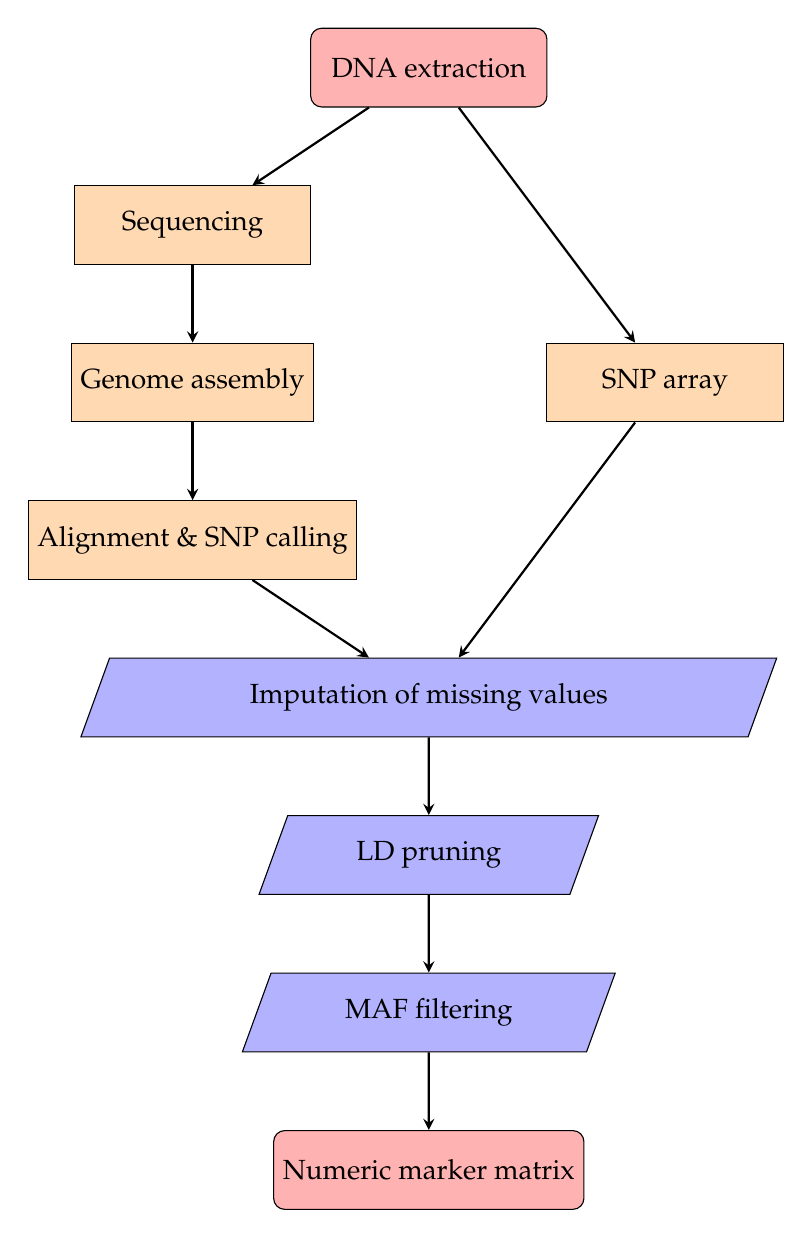
\begin{tikzpicture}[node distance=2cm]    
        \node (start) [startstop] {DNA extraction};
        \node (seq) [process, below of=start, xshift=-3cm] {Sequencing} ;
        \draw [arrow] (start) -- (seq);
        \node (SNP) [process, below of=start, xshift=3cm, yshift=-2cm] {SNP array} ;
        \draw [arrow] (start) -- (SNP);
        \node (ga) [process, below of=seq] {Genome assembly} ;
        \draw [arrow] (seq) -- (ga);
        \node (snpca) [process, below of=ga] {Alignment \& SNP calling} ;
        \draw [arrow] (ga) -- (snpca);
        \node (imp) [io, below of=snpca, xshift=3cm] {Imputation of missing values};
        \draw [arrow] (snpca) -- (imp) ;
        \draw [arrow] (SNP) -- (imp) ;
        \node (LD) [io, below of=imp] {LD pruning} ;
        \draw [arrow] (imp) -- (LD) ;
        \node (MAF) [io, below of=LD] {MAF filtering} ;
        \draw [arrow] (LD) -- (MAF) ;
        \node (bm) [startstop, below of=MAF] {Numeric marker matrix} ;
        \draw [arrow] (MAF) -- (bm) ;
      \end{tikzpicture}
        \caption[Schematic process of genotyping for quantitative genetics]{Schematic process of genotyping for quantitative genetics}
    \end{center}
  \end{small}
\end{figure}

Nothing here yet.

10000s of genome assemblies
Almost 1 million neural nets trained and the same amount of GWAS run.
Awesome stuff ! 



Recombination and LD in \textit{A. thaliana} \cite{kim2007recombination}
LD in \textit{A. thaliana} \cite{nordborg2002extent}
Evolution of selfing \cite{tang2007evolution}
Evolution and genetic differentiation among relatives of Arabidopsis thaliana \cite{koch2007evolution}
FLC haplotypes \cite{li2014multiple}


\begin{figure}[th]
\centering
\includegraphics[height=.55\textheight, width=1.1\textwidth]{Figures/plot_NAs_AT}
\decoRule
\caption[Haplotype structure on a 1kb window of chromosome 4 of
\textit{A. thaliana}]{Number of segregating haplotypes with a polymorphism in at least one
  position over a stretch of 1 kbp.}
\label{fig:chr_jul}
\end{figure}
\cite{dittberner2018natural}

%----------------------------------------------------------------------------------------
%	THESIS CONTENT - APPENDICIES
%----------------------------------------------------------------------------------------
\appendix % Cue to tell LaTeX that the following "chapters" are Appendices
% Include the appendices of the thesis as separate files from the Appendices folder
% Uncomment the lines as you writethe Appendices
% Appendix A

\chapter{Source code GWAS-Flow} % Main appendix title

\label{AppendixA} % For referencing this appendix elsewhere, use \ref{AppendixA}


\linespread{1.5} 
\section{gwas.py}
\begin{lstlisting}[language=Python]
import os
import sys
import time
import numpy as np
import pandas as pd
import main
import h5py

# set defaults 
mac_min = 1
batch_size =  500000 
out_file = "results.csv"
m = 'phenotype_value'
perm = 1
mac_min= 6

X_file = 'gwas_sample_data/AT_geno.hdf5'
Y_file = 'gwas_sample_data/phenotype.csv'
K_file = 'gwas_sample_data/kinship_ibs_binary_mac5.h5py'



for i in range (1,len(sys.argv),2):
    if sys.argv[i] == "-x" or sys.argv[i] == "--genotype":
        X_file = sys.argv[i+1]
    elif sys.argv[i] == "-y" or sys.argv[i] == "--phenotype":
        Y_file = sys.argv[i+1]
    elif sys.argv[i] == "-k" or sys.argv[i] == "--kinship":
        K_file = sys.argv[i+1]
    elif sys.argv[i] == "-m":
        m = sys.argv[i+1]
    elif sys.argv[i] == "-a" or sys.argv[i] == "--mac_min":
        mac_min = int(sys.argv[i+1])
    elif sys.argv[i] == "-bs" or sys.argv[i] == "--batch-size":
        batch_size = int(sys.argv[i+1])
    elif sys.argv[i] == "-p" or sys.argv[i] == "--perm":
        perm  = int(sys.argv[i+1])
    elif sys.argv[i] == "-o" or sys.argv[i] == "--out":
        out_file = sys.argv[i+1]
    elif sys.argv[i] == "-h" or sys.argv[i] == "--help":
        print("-x , --genotype :file containing marker information in csv or hdf5 format of size")
        print("-y , --phenotype: file container phenotype information in csv format"  )
        print("-k , --kinship : file containing kinship matrix of size k X k in csv or hdf5 format")
        print("-m : name of columnn containing the phenotype : default m = phenotype_value")
        print("-a , --mac_min : integer specifying the minimum minor allele count necessary for a marker to be included. Default a = 1" )
        print("-bs, --batch-size : integer specifying the number of markers processed at once. Default -bs 500000" )
        print("-p , --perm : single integer specifying the number of permutations. Default 1 == no perm ")
        print("-o , --out : name of output file. Default -o results.csv  ")
        print("-h , --help : prints help and command line options")
        quit()
    else:
        print('unknown option ' + str(sys.argv[i]))
        quit()



print("parsed commandline args")

start = time.time()

X,K,Y_,markers = main.load_and_prepare_data(X_file,Y_file,K_file,m)


## MAF filterin
markers_used , X , macs = main.mac_filter(mac_min,X,markers)

## prepare
print("Begin performing GWAS on ", Y_file)

if perm == 1:
    output = main.gwas(X,K,Y_,batch_size)   
    if( X_file.split(".")[-1] == 'csv'):
        chr_pos = np.array(list(map(lambda x : x.split("- "),markers_used)))
    else: 
        chr_reg = h5py.File(X_file,'r')['positions'].attrs['chr_regions']
        mk_index= np.array(range(len(markers)),dtype=int)[macs >= mac_min]
        chr_pos = np.array([list(map(lambda x: sum(x > chr_reg[:,1]) + 1, mk_index)), markers_used]).T
        my_time = np.repeat((time.time()-start),len(chr_pos))
    pd.DataFrame({
        'chr' : chr_pos[:,0] ,
        'pos' : chr_pos[:,1] , 
        'pval': output[:,0] ,
        'mac' : np.array(macs[macs >= mac_min],dtype=np.int) ,
        'eff_size': output[:,1] ,
        'SE' : output[:,2]}).to_csv(out_file,index=False)
elif perm > 1:
    min_pval = []
    perm_seeds = []
    my_time = []
    for i in range(perm):
        start_perm = time.time()
        print("Running permutation ", i+1, " of ",perm)
        my_seed  = np.asscalar(np.random.randint(9999,size=1))
        perm_seeds.append(my_seed)
        np.random.seed(my_seed)
        Y_perm = np.random.permutation(Y_)
        output = main.gwas(X,K,Y_perm,batch_size)
        min_pval.append(np.min(output[:,0]))
        print("Elapsed time for permuatation",i+1 ," with p_min", min_pval[i]," is",": ", round(time.time() - start_perm,2))
        my_time.append(time.time()-start_perm)
    pd.DataFrame({
        'time': my_time ,
        'seed': perm_seeds ,
        'min_p': min_pval }).to_csv(out_file,index=False)

print("done")
 
end = time.time()
eltime = np.round(end -start,2)

if eltime <= 59:
    print("Total time elapsed",  eltime, "seconds")
elif eltime > 59 and eltime <= 3600:
    print("Total time elapsed",  np.round(eltime / 60,2) , "minutes")
elif eltime > 3600 :
    print("Total time elapsed",  np.round(eltime / 60 / 60,2), "hours")

  \end{lstlisting}



  \section{main.py}
  \begin{lstlisting}[language=Python]
    import pandas as pd 
    import numpy as np
    from scipy.stats import f
    import tensorflow as tf
    import limix
    import herit
    import h5py
    import limix
    import multiprocessing as mlt

    def load_and_prepare_data(X_file,Y_file,K_file,m):
    type_K = K_file.split(".")[-1]
    type_X = X_file.split(".")[-1]
    
    ## load and preprocess genotype matrix 
    Y = pd.read_csv(Y_file,engine='python').sort_values(['accession_id']).groupby('accession_id').mean()
    Y = pd.DataFrame({'accession_id' :  Y.index, 'phenotype_value' : Y[m]})
    if type_X == 'hdf5' or type_X == 'h5py'  :
        SNP = h5py.File(X_file,'r')
        markers= np.asarray(SNP['positions'])
        acc_X =  np.asarray(SNP['accessions'][:],dtype=np.int)
    elif type_X == 'csv' :
        X = pd.read_csv(X_file,index_col=0)
        markers = X.columns.values
        acc_X = X.index
        X = np.asarray(X,dtype=np.float32)/2
    else :
        sys.exit("Only hdf5, h5py and csv files are supported")
      
    if type_K == 'hdf5' or type_K == 'h5py':
        k = h5py.File(K_file,'r')
        acc_K = np.asarray(k['accessions'][:],dtype=np.int)
    elif type_K == 'csv':
        k = pd.read_csv(K_file,index_col=0)
        acc_K = k.index
        k = np.array(k, dtype=np.float32)

    acc_Y =  np.asarray(Y[['accession_id']]).flatten()
    acc_isec = [isec for isec in acc_X if isec in acc_Y]
        
    idx_acc = list(map(lambda x: x in acc_isec, acc_X))
    idy_acc = list(map(lambda x: x in acc_isec, acc_Y))
    idk_acc = list(map(lambda x: x in acc_isec, acc_K))

    Y_ = np.asarray(Y.drop('accession_id',1),dtype=np.float32)[idy_acc,:]

    if type_X == 'hdf5' or type_X == 'h5py' :
        X = np.asarray(SNP['snps'][0:(len(SNP['snps'])+1),],dtype=np.float32)[:,idx_acc].T
        X = X[np.argsort(acc_X[idx_acc]),:]
        k1 = np.asarray(k['kinship'][:])[idk_acc,:]
        K  = k1[:,idk_acc]
        K = K[np.argsort(acc_X[idx_acc]),:]
        K = K[:,np.argsort(acc_X[idx_acc])]
    else:
        X  = X[idx_acc,:]
        k1 = k[idk_acc,:]
        K  = k1[:,idk_acc]
        
       
    print("data has been imported")
    return X,K,Y_,markers


def mac_filter(mac_min, X, markers):
    ac1 = np.sum(X,axis=0)
    ac0 = X.shape[0] - ac1
    macs = np.minimum(ac1,ac0)
    markers_used  = markers[macs >= mac_min]
    X = X[:,macs >= mac_min]
    return markers_used, X, macs

def gwas(X,K,Y,batch_size):
    n_marker = X.shape[1]
    n = len(Y)
    ## REML   
    K_stand = (n-1)/np.sum((np.identity(n) - np.ones((n,n))/n) * K) * K
    vg, delta, ve  = herit.estimate(Y,"normal",K_stand,verbose = False)
    print(" Pseudo-heritability is " , vg / (ve + vg + delta))
    print(" Performing GWAS on ", n , " phenotypes and ", n_marker ,"markers")
    ## Transform kinship-matrix, phenotypes and estimate intercpt
    Xo = np.ones(K.shape[0]).flatten()
    M = np.transpose(np.linalg.inv(np.linalg.cholesky(vg * K_stand + ve  * np.identity(n)))).astype(np.float32)
    Y_t = np.sum(np.multiply(np.transpose(M),Y),axis=1).astype(np.float32)
    int_t = np.sum(np.multiply(np.transpose(M),np.ones(n)),axis=1).astype(np.float32)
    ## EMMAX Scan
    RSS_env = (np.linalg.lstsq(np.reshape(int_t,(n,-1)) , np.reshape(Y_t,(n,-1)))[1]).astype(np.float32)
    ## calculate betas and se of betas 
    def stderr(a,M,Y_t2d,int_t):
         x = tf.stack((int_t,tf.squeeze(tf.matmul(M.T,tf.reshape(a,(n,-1))))),axis=1)
         coeff = tf.matmul(tf.matmul(tf.linalg.inv(tf.matmul(tf.transpose(x),x)),tf.transpose(x)),Y_t2d)
         SSE = tf.reduce_sum(tf.math.square(tf.math.subtract(Y_t,tf.math.add(tf.math.multiply(x[:,1],coeff[0,0]),tf.math.multiply(x[:,1],coeff[1,0])))))
         SE = tf.math.sqrt(SSE/(471-(1+2)))
         StdERR = tf.sqrt(tf.linalg.diag_part(tf.math.multiply(SE , tf.linalg.inv(tf.matmul(tf.transpose(x),x)))))[1]
         return tf.stack((coeff[1,0],StdERR))
    ## calculate residual sum squares 
    def rss(a,M,y,int_t):
         x_t = tf.reduce_sum(tf.math.multiply(M.T,a),axis=1)
         lm_res = tf.linalg.lstsq(tf.transpose(tf.stack((int_t,x_t),axis=0)),Y_t2d)
         lm_x = tf.concat((tf.squeeze(lm_res),x_t),axis=0)
         return tf.reduce_sum(tf.math.square(tf.math.subtract(tf.squeeze(Y_t2d),tf.math.add(tf.math.multiply(lm_x[1],lm_x[2:]), tf.multiply(lm_x[0],int_t)))))
    ## loop over the batches 
    for i in range(int(np.ceil(n_marker/batch_size))):
        tf.reset_default_graph()
        if n_marker < batch_size:
            X_sub = X
        else:
            lower_limit = batch_size * i 
            upper_limit = batch_size * i + batch_size
            if upper_limit <= n_marker :
                X_sub = X[:,lower_limit:upper_limit]
                print("Working on markers ", lower_limit , " to ", upper_limit, " of ", n_marker )    
            else:
                X_sub = X[:,lower_limit:]
                print("Working on markers ", lower_limit , " to ", n_marker, " of ", n_marker )    
        config = tf.ConfigProto()
        n_cores = mlt.cpu_count()
        config.intra_op_parallelism_threads = n_cores
        config.inter_op_parallelism_threads = n_cores
        sess = tf.Session(config=config)                                             
        Y_t2d = tf.cast(tf.reshape(Y_t,(n,-1)),dtype=tf.float32)                     
        y_tensor =  tf.convert_to_tensor(Y_t,dtype = tf.float32)                                      
        StdERR = tf.map_fn(lambda a : stderr(a,M,Y_t2d,int_t), X_sub.T)              
        R1_full = tf.map_fn(lambda a: rss(a,M,Y_t2d,int_t), X_sub.T)
        F_1 = tf.divide(tf.subtract(RSS_env, R1_full),tf.divide(R1_full,(n-3)))
        if i == 0 :
            output = sess.run(tf.concat([tf.reshape(F_1,(X_sub.shape[1],-1)),StdERR],axis=1))
        else :
            tmp = sess.run(tf.concat([tf.reshape(F_1,(X_sub.shape[1],-1)),StdERR],axis=1))
            output = np.append(output,tmp,axis=0)
        sess.close()
        F_dist = output[:,0]
    pval  = 1 - f.cdf(F_dist,1,n-3)
    output[:,0] = pval
    return output 


  \end{lstlisting}

\section{herit.py}
\begin{lstlisting}[language=Python]
  
def estimate(y, lik, K, M=None, verbose=True):
    from numpy_sugar.linalg import economic_qs
    from numpy import pi, var, diag
    from glimix_core.glmm import GLMMExpFam
    from glimix_core.lmm import LMM
    from limix._data._assert import assert_likelihood
    from limix._data import normalize_likelihood, conform_dataset 
    from limix.qtl._assert import assert_finite
    from limix._display import session_block, session_line
    lik = normalize_likelihood(lik)
    lik_name = lik[0]
    with session_block("Heritability analysis", disable=not verbose):
        with session_line("Normalising input...", disable=not verbose):
            data = conform_dataset(y, M=M, K=K)
        y = data["y"]
        M = data["M"]
        K = data["K"]
        assert_finite(y, M, K)
        if K is not None:
           # K = K / diag(K).mean()
            QS = economic_qs(K)
        else:
            QS = None
        if lik_name == "normal":
            method = LMM(y.values, M.values, QS, restricted=True)
            method.fit(verbose=verbose)
        else:
            method = GLMMExpFam(y, lik, M.values, QS, n_int=500)
            method.fit(verbose=verbose, factr=1e6, pgtol=1e-3)
        g = method.scale * (1 - method.delta)
        e = method.scale * method.delta
        if lik_name == "bernoulli":
            e += pi * pi / 3
        v = var(method.mean())
        return g , v , e 


\end{lstlisting} 
% Appendix Template

\chapter{\textit{A. thaliana} phenotypic data} % Main appendix title
\label{AppendixB} % Change X to a consecutive letter; for referencing this appendix elsewhere, use \ref{AppendixX}

\begin{longtable}{p{.07\textwidth} p{.34\textwidth} p{.30\textwidth} p{.35\textwidth}}
  \toprule
  ID & Phenotype name & doi & Reference \\
  \midrule
 1 & FT Diameter Field & 10.21958/phenotype:1 & \cite{atwell2010}\\
 2 & At2 CFU2 & 10.21958/phenotype:2 & \cite{atwell2010}\\
 3 & Leaf serr 16 & 10.21958/phenotype:3 & \cite{atwell2010}\\
 4 & Seed bank 133-91 & 10.21958/phenotype:4 & \cite{atwell2010}\\
 5 & Na23 & 10.21958/phenotype:5 & \cite{atwell2010}\\
 6 & Leaf serr 10 & 10.21958/phenotype:6 & \cite{atwell2010}\\
 7 & Emco5 & 10.21958/phenotype:7 & \cite{atwell2010}\\
 8 & Leaf roll 16 & 10.21958/phenotype:8 & \cite{atwell2010}\\
 9 & Leaf roll 10 & 10.21958/phenotype:9 & \cite{atwell2010}\\
 10 & Bs & 10.21958/phenotype:10 & \cite{atwell2010}\\
 11 & 2W & 10.21958/phenotype:11 & \cite{atwell2010}\\
 12 & Rosette Erect 22 & 10.21958/phenotype:12 & \cite{atwell2010}\\
 13 & Cd114 & 10.21958/phenotype:13 & \cite{atwell2010}\\
 14 & Width 16 & 10.21958/phenotype:14 & \cite{atwell2010}\\
 15 & Storage 28 days & 10.21958/phenotype:15 & \cite{atwell2010}\\
 16 & LY & 10.21958/phenotype:16 & \cite{atwell2010}\\
 17 & avrRpm1 & 10.21958/phenotype:17 & \cite{atwell2010}\\
 18 & Width 10 & 10.21958/phenotype:18 & \cite{atwell2010}\\
 19 & Chlorosis 22 & 10.21958/phenotype:19 & \cite{atwell2010}\\
 20 & Storage 7 days & 10.21958/phenotype:20 & \cite{atwell2010}\\
 21 & As2 CFU2 & 10.21958/phenotype:21 & \cite{atwell2010}\\
 22 & Co59 & 10.21958/phenotype:22 & \cite{atwell2010}\\
 23 & FW & 10.21958/phenotype:23 & \cite{atwell2010}\\
 24 & Cu65 & 10.21958/phenotype:24 & \cite{atwell2010}\\
 25 & Bacterial titer & 10.21958/phenotype:25 & \cite{atwell2010}\\
 26 & Width 22 & 10.21958/phenotype:26 & \cite{atwell2010}\\
 27 & Storage 56 days & 10.21958/phenotype:27 & \cite{atwell2010}\\
 28 & YEL & 10.21958/phenotype:28 & \cite{atwell2010}\\
 29 & FLC & 10.21958/phenotype:29 & \cite{atwell2010}\\
 30 & FT16 & 10.21958/phenotype:30 & \cite{atwell2010}\\
 31 & FT10 & 10.21958/phenotype:31 & \cite{atwell2010}\\
 32 & FT Duration GH & 10.21958/phenotype:32 & \cite{atwell2010}\\
 33 & Se82 & 10.21958/phenotype:33 & \cite{atwell2010}\\
 34 & LDV & 10.21958/phenotype:34 & \cite{atwell2010}\\
 35 & Noco2 & 10.21958/phenotype:35 & \cite{atwell2010}\\
 36 & 8W GH LN & 10.21958/phenotype:36 & \cite{atwell2010}\\
 37 & 0W & 10.21958/phenotype:37 & \cite{atwell2010}\\
 38 & MT GH & 10.21958/phenotype:38 & \cite{atwell2010}\\
 39 & After Vern Growth & 10.21958/phenotype:39 & \cite{atwell2010}\\
 40 & Aphid number & 10.21958/phenotype:40 & \cite{atwell2010}\\
 41 & LN22 & 10.21958/phenotype:41 & \cite{atwell2010}\\
 42 & Bs CFU2 & 10.21958/phenotype:42 & \cite{atwell2010}\\
 43 & avrRpt2 & 10.21958/phenotype:43 & \cite{atwell2010}\\
 44 & Hypocotyl length & 10.21958/phenotype:44 & \cite{atwell2010}\\
 45 & Germ 22 & 10.21958/phenotype:45 & \cite{atwell2010}\\
 46 & Leaf roll 22 & 10.21958/phenotype:46 & \cite{atwell2010}\\
 47 & SD & 10.21958/phenotype:47 & \cite{atwell2010}\\
 48 & 8W & 10.21958/phenotype:48 & \cite{atwell2010}\\
 49 & FT GH & 10.21958/phenotype:49 & \cite{atwell2010}\\
 50 & DSDS50 & 10.21958/phenotype:50 & \cite{atwell2010}\\
 51 & Ca43 & 10.21958/phenotype:51 & \cite{atwell2010}\\
 52 & LC Duration GH & 10.21958/phenotype:52 & \cite{atwell2010}\\
 53 & 0W GH FT & 10.21958/phenotype:53 & \cite{atwell2010}\\
 54 & B11 & 10.21958/phenotype:54 & \cite{atwell2010}\\
 55 & Chlorosis 10 & 10.21958/phenotype:55 & \cite{atwell2010}\\
 56 & RP GH & 10.21958/phenotype:56 & \cite{atwell2010}\\
 57 & Chlorosis 16 & 10.21958/phenotype:57 & \cite{atwell2010}\\
 58 & LFS GH & 10.21958/phenotype:58 & \cite{atwell2010}\\
 59 & Germ 10 & 10.21958/phenotype:59 & \cite{atwell2010}\\
 60 & Germ 16 & 10.21958/phenotype:60 & \cite{atwell2010}\\
 61 & Anthocyanin 16 & 10.21958/phenotype:61 & \cite{atwell2010}\\
 62 & Anthocyanin 10 & 10.21958/phenotype:62 & \cite{atwell2010}\\
 63 & At1 CFU2 & 10.21958/phenotype:63 & \cite{atwell2010}\\
 64 & Ni60 & 10.21958/phenotype:64 & \cite{atwell2010}\\
 65 & P31 & 10.21958/phenotype:65 & \cite{atwell2010}\\
 66 & Emwa1 & 10.21958/phenotype:66 & \cite{atwell2010}\\
 67 & As75 & 10.21958/phenotype:67 & \cite{atwell2010}\\
 68 & Germ in dark & 10.21958/phenotype:68 & \cite{atwell2010}\\
 69 & FRI & 10.21958/phenotype:69 & \cite{atwell2010}\\
 70 & As CFU2 & 10.21958/phenotype:70 & \cite{atwell2010}\\
 71 & Trichome avg C & 10.21958/phenotype:71 & \cite{atwell2010}\\
 72 & Vern Growth & 10.21958/phenotype:72 & \cite{atwell2010}\\
 73 & Mo98 & 10.21958/phenotype:73 & \cite{atwell2010}\\
 74 & Hiks1 & 10.21958/phenotype:74 & \cite{atwell2010}\\
 75 & Anthocyanin 22 & 10.21958/phenotype:75 & \cite{atwell2010}\\
 76 & Zn66 & 10.21958/phenotype:76 & \cite{atwell2010}\\
 77 & Trichome avg JA & 10.21958/phenotype:77 & \cite{atwell2010}\\
 78 & LES & 10.21958/phenotype:78 & \cite{atwell2010}\\
 79 & Silique 16 & 10.21958/phenotype:79 & \cite{atwell2010}\\
 80 & Emoy* & 10.21958/phenotype:80 & \cite{atwell2010}\\
 81 & K39 & 10.21958/phenotype:81 & \cite{atwell2010}\\
 82 & 0W GH LN & 10.21958/phenotype:82 & \cite{atwell2010}\\
 83 & At2 & 10.21958/phenotype:83 & \cite{atwell2010}\\
 84 & At1 & 10.21958/phenotype:84 & \cite{atwell2010}\\
 85 & LN10 & 10.21958/phenotype:85 & \cite{atwell2010}\\
 86 & FT Field & 10.21958/phenotype:86 & \cite{atwell2010}\\
 87 & LN16 & 10.21958/phenotype:87 & \cite{atwell2010}\\
 88 & avrB & 10.21958/phenotype:88 & \cite{atwell2010}\\
 89 & LD & 10.21958/phenotype:89 & \cite{atwell2010}\\
 90 & Seedling Growth & 10.21958/phenotype:90 & \cite{atwell2010}\\
 91 & S34 & 10.21958/phenotype:91 & \cite{atwell2010}\\
 92 & Leaf serr 22 & 10.21958/phenotype:92 & \cite{atwell2010}\\
 93 & DW & 10.21958/phenotype:93 & \cite{atwell2010}\\
 94 & Seed Dormancy & 10.21958/phenotype:94 & \cite{atwell2010}\\
 95 & Mn55 & 10.21958/phenotype:95 & \cite{atwell2010}\\
 96 & Silique 22 & 10.21958/phenotype:96 & \cite{atwell2010}\\
 97 & avrPphB & 10.21958/phenotype:97 & \cite{atwell2010}\\
 98 & Fe56 & 10.21958/phenotype:98 & \cite{atwell2010}\\
 99 & 8W GH FT & 10.21958/phenotype:99 & \cite{atwell2010}\\
 100 & 4W & 10.21958/phenotype:100 & \cite{atwell2010}\\
 101 & Li7 & 10.21958/phenotype:101 & \cite{atwell2010}\\
 102 & FT22 & 10.21958/phenotype:102 & \cite{atwell2010}\\
 103 & As2 & 10.21958/phenotype:103 & \cite{atwell2010}\\
 104 & SDV & 10.21958/phenotype:104 & \cite{atwell2010}\\
 105 & Mg25 & 10.21958/phenotype:105 & \cite{atwell2010}\\
 106 & Secondary Dormancy & 10.21958/phenotype:106 & \cite{atwell2010}\\
 107 & As & 10.21958/phenotype:107 & \cite{atwell2010}\\
 108 & Area Sweden 2009 (1st experiment) & 10.21958/phenotype:108 & \cite{li2010}\\
 109 & Size Planting Summer 2009 & 10.21958/phenotype:109 & \cite{li2010}\\
 110 & Size Sweden 2009 (2nd experiment) & 10.21958/phenotype:110 & \cite{li2010}\\
 111 & Size Planting Summer Loc Sweden 2009 & 10.21958/phenotype:111 & \cite{li2010}\\
 112 & Area Sweden 2009 (2nd experiment) & 10.21958/phenotype:112 & \cite{li2010}\\
 113 & DTF Sweden 2008 (1st experiment) & 10.21958/phenotype:113 & \cite{li2010}\\
 114 & Yield Sweden 2009 (2nd experiment) & 10.21958/phenotype:114 & \cite{li2010}\\
 115 & Size Loc Sweden 2009 & 10.21958/phenotype:115 & \cite{li2010}\\
 116 & DTF planting Summer Loc Sweden 2009 & 10.21958/phenotype:116 & \cite{li2010}\\
 117 & DTF loc Sweden 2008 & 10.21958/phenotype:117 & \cite{li2010}\\
 118 & DTF loc Sweden 2009 & 10.21958/phenotype:118 & \cite{li2010}\\
 119 & DTF Spain 2009 (1st experiment) & 10.21958/phenotype:119 & \cite{li2010}\\
 120 & DTF planting Loc 2008 & 10.21958/phenotype:120 & \cite{li2010}\\
 121 & DTF Spain 2009 (2nd experiment) & 10.21958/phenotype:121 & \cite{li2010}\\
 122 & Yield Spain 2009 (2nd experiment) & 10.21958/phenotype:122 & \cite{li2010}\\
 123 & Size Sweden 2009 (1st experiment) & 10.21958/phenotype:123 & \cite{li2010}\\
 124 & Yield Spain 2009 (1st experiment) & 10.21958/phenotype:124 & \cite{li2010}\\
 125 & DTF main Effect 2009 & 10.21958/phenotype:125 & \cite{li2010}\\
 126 & DTF main Effect 2008 & 10.21958/phenotype:126 & \cite{li2010}\\
 127 & Size Spain 2009 (2nd experiment) & 10.21958/phenotype:127 & \cite{li2010}\\
 128 & Size Spain 2009 (1st experiment) & 10.21958/phenotype:128 & \cite{li2010}\\
 129 & DTF planting Summer 2009 & 10.21958/phenotype:129 & \cite{li2010}\\
 130 & DTF planting Summer 2008 & 10.21958/phenotype:130 & \cite{li2010}\\
 131 & Size Main Effect 2009 & 10.21958/phenotype:131 & \cite{li2010}\\
 132 & DTF Spain 2008 (1st experiment) & 10.21958/phenotype:132 & \cite{li2010}\\
 133 & Yield Planting Summer 2009 & 10.21958/phenotype:133 & \cite{li2010}\\
 134 & DTF Sweden 2009 (1st experiment) & 10.21958/phenotype:134 & \cite{li2010}\\
 135 & Yield Loc Sweden 2009 & 10.21958/phenotype:135 & \cite{li2010}\\
 136 & DTF Spain 2008 (2nd experiment) & 10.21958/phenotype:136 & \cite{li2010}\\
 137 & Yield Main Effect 2009 & 10.21958/phenotype:137 & \cite{li2010}\\
 138 & Yield Planting Summer Loc Sweden 009 & 10.21958/phenotype:138 & \cite{li2010}\\
 139 & Yield Sweden 2009 (1st experiment) & 10.21958/phenotype:139 & \cite{li2010}\\
 140 & DTF Sweden 2009 (2nd experiment) & 10.21958/phenotype:140 & \cite{li2010}\\
 141 & DTF Sweden 2008 (2nd experiment) & 10.21958/phenotype:141 & \cite{li2010}\\
 142 & Mature cell length & 10.21958/phenotype:142 & \cite{me2014}\\
 143 & Meristem zone length & 10.21958/phenotype:143 & \cite{me2014}\\
 144 & M216T665 & 10.21958/phenotype:144 & \cite{strauch2015}\\
 145 & M130T666 & 10.21958/phenotype:145 & \cite{strauch2015}\\
 146 & M172T666 & 10.21958/phenotype:146 & \cite{strauch2015}\\
 261 & FT10 & 10.21958/phenotype:261 &\cite{1001genome}\\
 262 & FT16 & 10.21958/phenotype:262 &\cite{1001genome}\\
 269 & Li7 & 10.21958/phenotype:269 & \cite{ion2015}\\
 270 & B11 & 10.21958/phenotype:270 & \cite{ion2015}\\
 271 & Na23 & 10.21958/phenotype:271 & \cite{ion2015}\\
 272 & Mg25 & 10.21958/phenotype:272 & \cite{ion2015}\\
 273 & P31 & 10.21958/phenotype:273 & \cite{ion2015}\\
 274 & S34 & 10.21958/phenotype:274 & \cite{ion2015}\\
 275 & K39 & 10.21958/phenotype:275 & \cite{ion2015}\\
 276 & Ca43 & 10.21958/phenotype:276 & \cite{ion2015}\\
 277 & Mn55 & 10.21958/phenotype:277 & \cite{ion2015}\\
 279 & Co59 & 10.21958/phenotype:279 & \cite{ion2015}\\
 280 & Ni60 & 10.21958/phenotype:280 & \cite{ion2015}\\
 281 & Cu65 & 10.21958/phenotype:281 & \cite{ion2015}\\
 282 & Zn66 & 10.21958/phenotype:282 & \cite{ion2015}\\
 283 & As75 & 10.21958/phenotype:283 & \cite{ion2015}\\
 284 & Se82 & 10.21958/phenotype:284 & \cite{ion2015}\\
\bottomrule
\end{longtable}

%% Appendix A


\chapter{Genomic prediction} % Main appendix title

\label{AppendixC} % For referencing this appendix elsewhere, use \ref{AppendixA}

\section{GP ANN}
\begin{lstlisting}[language=Python]

  import os,sys,gc
import pandas as pd
import numpy as np
import timeit
from datetime import datetime
import keras
import tensorflow as tf
from keras import backend as K
from keras import layers
from keras.models import Sequential
from keras.layers import Dense, Dropout, GaussianNoise, AlphaDropout, Reshape
from keras.layers import Flatten, LocallyConnected1D, LocallyConnected2D
from keras.optimizers import Adam, Adagrad, Adadelta
from keras.backend.tensorflow_backend import set_session 

##set default values

learning_rate = 0.01
JobID = 1
ps = 25
optim = "adam"
X_file = "KE.geno.csv"
Y_file = "KE_pheno.csv"
CV_file = "KE_cv_pw.csv"
label = "DtSILK"
start_time = timeit.default_timer()
act="relu"
drop_rate = str('0.5,0.5,0.5')
arc = str('63,63')
DG = 'D,D,D,D,D,G'
LC = True
training_epochs = 25
hyp = False

### parse command line arguments

for i in range (1,len(sys.argv),2):
    if sys.argv[i] == "-x":
        X_file = sys.argv[i+1]
    elif sys.argv[i] == "-y":
        Y_file = sys.argv[i+1]
    elif sys.argv[i] == "-cv":
        CV_file = sys.argv[i+1]
    elif sys.argv[i] == "-JobID":
        JobID = int(sys.argv[i+1])
    elif sys.argv[i] == "-label":
        label = sys.argv[i+1]
    elif sys.argv[i] == "-act":
        act = str(sys.argv[i+1])
    elif sys.argv[i] == "-epochs":
        training_epochs = int(sys.argv[i+1])
    elif sys.argv[i] == "-lr":
        learning_rate = float(sys.argv[i+1])
    elif sys.argv[i] == "-arc":
        arc = sys.argv[i+1]
    elif sys.argv[i] == "-ps":
        ps = int(sys.argv[i+1])
    elif sys.argv[i] == "-dr":
        drop_rate=str(sys.argv[i+1])
    elif sys.argv[i] == "-LC":
         LC = bool(sys.argv[i+1])
    elif sys.argv[i] == "hyp":
        hyp = bool(sys.argv[i+1])
    else:
        print('unknown option ' + str(sys.argv[i]))
        quit()

        
        
## change dir to data location


#os.chdir('/home/jaf81qa/jan_storage/tens')
x = pd.read_csv(X_file, index_col = 0)
#os.chdir("/storage/full-share/genoPred/maze")
y = pd.read_csv(Y_file, index_col = 0)
cv_folds = pd.read_csv(CV_file,index_col=0)

## select column of phenotype file via columnname

y = y[[label]]
## activity_regularizer=regularizers.l1(0.01)))

def build_network(arc,drop_rate,LC,DG):
    def add_drops(model,drop_out,k):
        if DG[k].upper() == 'D':
            model.add(Dropout(drop_out[0]))
        elif DG[k].upper() == 'G':
            model.add(GaussianNoise(drop_out[k]))
        elif DG[k].upper() == "A":
            model.add(AlphaDropout(drop_out[k]))
        else:
            pass
        return model    
    DG = DG.strip().split(",")
    arc = arc.strip().split(",")
    archit = []
    for layer in  arc:
        archit.append(int(layer))
    layer_number = len(archit)        
    drop_rate = drop_rate.strip().split(",")
    drop_out = []
    for drops in drop_rate:
        drop_out.append(float(drops)) 
    model = Sequential()
    if LC == True:
        model.add(Reshape(input_shape=(x_train.shape[1],),target_shape=(x_train.shape[1],1)))
        model.add(LocallyConnected1D(1,10,strides=7,input_shape=(x_train.shape[1],1)))
        model.add(Flatten())
        start = 0
        model = add_drops(model,drop_out,start)
    elif LC == False:
        model.add(Dense(archit[0], kernel_initializer='truncated_normal', activation=act, input_shape=(x_train.shape[1],)))
        model = add_drops(model,drop_out,start)
    start = 1
    for k in range(start,len(archit)):
        model.add(Dense(archit[k], kernel_initializer='truncated_normal', activation=act))
        model = add_drops(model,drop_out,k)
    model.add(Dense(1, kernel_initializer='truncated_normal'))
    return(model)

     
config = tf.ConfigProto()
#config.gpu_options.per_process_gpu_memory_fraction = 0.1
config.gpu_options.allow_growth = True
set_session(tf.Session(config=config))


if not os.path.isfile("RESULTScv50.txt"):
    out2 = open("RESULTScv50.txt",'w')
    out2.write('DateTime\tCompTime\tDF\tGenos\tPhenos\tCV_fold\tArchit\tConv\tActFun\tEpochs\tdrop_rate\tAccuracy\n' )

    
for k in range(1,51):
    print("Training on cv fold "+ str(k))
    cv = cv_folds['cv_' + str(k)]
    num_cvs = np.ptp(cv) + 1
    
    i = 1
    x_train = x[cv != i] 
    x_test = x[cv == i] 
    y_train = y[cv != i]
    y_test = y[cv == i]

    yhat = np.zeros(shape = y_test.shape)

    model = build_network(arc,drop_rate,LC,DG)
    model.compile(loss='mse', optimizer=Adam(lr=0.01,decay = 0.001),metrics=['accuracy'])
    model.fit(x_train,y_train, epochs=training_epochs , verbose=0) 
#    score = model.evaluate(x_test, y_test, verbose=0)
    bla = model.predict(x_test)
    y_sub= y[np.asarray(cv == i)]
    
    print(model.summary())
    print('\n')
    print(label)        

    comp_time = int(round(timeit.default_timer() - start_time,0))

    DateTime = datetime.now().strftime('%Y-%m-%d %H:%M:%S')
    acc = np.corrcoef(bla[:,0],np.asarray(y_sub)[:,0])[0,1]

    out2 = open("RESULTScv50.txt", 'a')
    out2.write('%s\t%i\t%s\t%s\t%s\t%i\t%s\t%s\t%s\t%i\t%s\t%0.5f\n' % (
        DateTime, comp_time, label, X_file, Y_file, int(k), arc, LC,  act,int(training_epochs), drop_rate, round(acc,4)))

    del model,bla, x_train, x_test, y_train, y_test 
    K.clear_session() 
    gc.collect()
    
    config = tf.ConfigProto()
    #config.gpu_options.per_process_gpu_memory_fraction = 0.1
    config.gpu_options.allow_growth = True
    set_session(tf.Session(config=config))
\end{lstlisting}

\section{GBLUP script}
\begin{lstlisting}[language=R]
    geno_pred <- function(phenocsv,genocsv,cvfcsv,cvf=1,mod = "BRR",label,phe)
{
    my_phe <- phe
    depends<- c("BGLR","doBy","doParallel",'R.utils',"BBmisc","dplyr")
    foo <- sapply(depends,
                  function(X){if(!suppressPackageStartupMessages(require(X,character.only = T))){install.packages(X)}})
    foo <- sapply(depends,function(X){suppressPackageStartupMessages(library(X,character.only=TRUE))})
    rm(foo)
    
        
    maze <- read.csv(genocsv, row.names = 1)
    phe <- read.csv(phenocsv, row.names = 1)
    cvffolds <- read.csv(cvfcsv,row.names=1)
    
    X <- scale(maze)
    y <- phe[[label]]
    if(any(is.na(y))){
        rms <- which(is.na(y))
        y <- y[-rms]
        X <- X[-rms,]
    }
    for(i in 1:50){
        cvf = i
        n=length(y)
        seed <- sample(1:100,1)
                                        #set.seed(seed)
                                        #folds=sample(1:cvf,size=n,replace=T)
        folds = cvffolds[,cvf]
        yHatCV=rep(NA,n)
        
        for(i in 1:max(folds)){
            cat("Predicting cv-fold ",i," of ", max(folds))
            tst=which(folds==i)
            yNA=y
            yNA[tst]=NA
            fm=BGLR(y=yNA,ETA=list(list(X=X,model=mod)),verbose =F ,nIter=7000,burnIn=1000)
            yHatCV[tst]=fm$yHat[tst]
            cat("   done\n")
        }
        
        my_cor <- cor(yHatCV,y,use = "complete.obs")
        print(c("Corrleation of GP", mod, my_cor))
        filename = paste0(my_phe,"_gp_results.csv")
        print(filename)
        if(!any(dir() == filename)){
            res <- matrix(ncol=8, nrow = 1) %>%
                setColNames(c("geno","pheno","cv_folds","seed","label", "cor","method","nmark"))
            res[1,] <- c(as.character(genocsv),as.character(phenocsv),as.character(cvf),as.character(seed),
                         as.character(label),as.character(my_cor),as.character(mod),dim(X)[2])
            print("#################")
	    print(res)
	    print("############")
            write.csv(res,filename)
        }else{
            res <- read.csv(filename,row.names = 1)
            for(i in 1:7){
                res[,i] <- as.character(res[,i])
            }
            res[dim(res)[1]+1,] <- c(as.character(genocsv),phenocsv,cvf,seed,as.character(label),my_cor,mod,dim(X)[2])
            write.csv(res,filename)
        }
    }
    
  }
## execute this script with: Rscript ex.gblup.r -x genofile -y phenofile -c cv file
source("~/PHD/Projects/gblup/bglr.r")


my.args <- commandArgs(trailingOnly = TRUE)
#my.args <- c("-x", "gent_geno.csv","-y" , "gent_pheno.csv")
### set defaults 
#cvf.name = NA

## parsing the command line options 
all.opts <- c("-x","-y","-label","-h","-cv","-phe")
for(i in 1:length(my.args)){
    if( i %% 2 == 1){
        if(!my.args[i] %in%  all.opts){
            cat("unknown option", my.args[i], "Use only", all.opts , "\n")
            cat("use -h for help \n")
            quit()
        }
    }    
    if(my.args[i] == "-x"){
        geno.name <- as.character(my.args[i+1])
    } else if(my.args[i] == "-y") {
        pheno.name <- as.character(my.args[i+1])
    } else if(my.args[i] == "-label") {
        my_ph <- as.character(my.args[i+1])
    } else if(my.args[i] == "-cv"){
        cv.name = as.character(my.args[i+1])
    } else if(my.args[i] == "-phe"){
        my_phe <- as.character(my.args[i+1])
    } else if(my.args[i] == "-h") {
        print(" This script takes as a minimum two intputs\n")
        print(" -x genotypefile")
        print(" -y phenotypefile ")
        print(" -cv cross-valiadtion file : is optional if none is specified random 5 fold cv will be used")
        print(" -JobID : specify column number to use in your cross validation file")
        print(" -label : use header of phenotype file column you want to use")
        quit()
    }
}


#pheno.name <- my.args[1]
#geno.name <- my.args[2]
#cvf.name <- my.args[3]

geno_pred(phenocsv = pheno.name,genocsv=geno.name, cvfcsv = cv.name, label=my_ph,mod = "BRR", phe =my_phe)



\end{lstlisting}

%$


\section{Results of GP} \label{AC:gp_res}
  
\begin{figure}[H]
  \centering \includegraphics[height=1.05\textheight, width=1.1\textwidth]{Figures/cor_plots_0}
  \decoRule
 \label{fig:bla}
\end{figure}

\begin{figure}[H]
  \centering \includegraphics[height=1.05\textheight, width=1.1\textwidth]{Figures/cor_plots_1}
  \decoRule
 \label{fig:bla}
\end{figure}

\begin{figure}[H]
  \centering \includegraphics[height=1.05\textheight, width=1.1\textwidth]{Figures/cor_plots_2}
  \decoRule
 \label{fig:bla}
\end{figure}

\begin{figure}[H]
  \centering \includegraphics[height=1.05\textheight, width=1.1\textwidth]{Figures/cor_plots_3}
  \decoRule
 \label{fig:bla}
\end{figure}

\begin{figure}[H]
  \centering \includegraphics[height=1.05\textheight, width=1.1\textwidth]{Figures/cor_plots_4}
  \decoRule
 \label{fig:bla}
\end{figure}

\begin{figure}[H]
  \centering \includegraphics[height=1.05\textheight, width=1.1\textwidth]{Figures/cor_plots_5}
  \decoRule
 \label{fig:bla}
\end{figure}

\begin{figure}[H]
  \centering \includegraphics[height=1.05\textheight, width=1.1\textwidth]{Figures/cor_plots_6}
  \decoRule
 \label{fig:bla}
\end{figure}

\begin{figure}[H]
  \centering \includegraphics[height=1.05\textheight, width=1.1\textwidth]{Figures/cor_plots_7}
  \decoRule
 \label{fig:bla}
\end{figure}

\begin{figure}[H]
  \centering \includegraphics[height=.35\textheight, width=.65\textwidth]{Figures/cor_plots_8}
  \decoRule
 \label{fig:bla}
\end{figure}

% Appendix Template

\chapter{Supplementary results} % Main appendix title

\label{AppendixD} % Change X to a consecutive letter; for referencing this appendix elsewhere, use \ref{AppendixX}

\section{Correlation plots of \textit{A. thaliana} GP}  \label{AC:gp_res}
  
\begin{figure}[H]
  \centering \includegraphics[height=1.05\textheight, width=1.1\textwidth]{Figures/cor_plots_0}
  \decoRule
 \label{fig:bla}
\end{figure}

\begin{figure}[H]
  \centering \includegraphics[height=1.05\textheight, width=1.1\textwidth]{Figures/cor_plots_1}
  \decoRule
 \label{fig:bla}
\end{figure}

\begin{figure}[H]
  \centering \includegraphics[height=1.05\textheight, width=1.1\textwidth]{Figures/cor_plots_2}
  \decoRule
 \label{fig:bla}
\end{figure}

\begin{figure}[H]
  \centering \includegraphics[height=1.05\textheight, width=1.1\textwidth]{Figures/cor_plots_3}
  \decoRule
 \label{fig:bla}
\end{figure}

\begin{figure}[H]
  \centering \includegraphics[height=1.05\textheight, width=1.1\textwidth]{Figures/cor_plots_4}
  \decoRule
 \label{fig:bla}
\end{figure}

\begin{figure}[H]
  \centering \includegraphics[height=1.05\textheight, width=1.1\textwidth]{Figures/cor_plots_5}
  \decoRule
 \label{fig:bla}
\end{figure}

\begin{figure}[H]
  \centering \includegraphics[height=1.05\textheight, width=1.1\textwidth]{Figures/cor_plots_6}
  \decoRule
 \label{fig:bla}
\end{figure}

\begin{figure}[H]
  \centering \includegraphics[height=1.05\textheight, width=1.1\textwidth]{Figures/cor_plots_7}
  \decoRule
 \label{fig:bla}
\end{figure}

\begin{figure}[H]
  \centering \includegraphics[height=.35\textheight, width=.65\textwidth]{Figures/cor_plots_8}
  \decoRule
 \label{fig:bla}
\end{figure}



\section{Haplotype structure of \textit{A. thaliana}} \label{haplo:str}

\begin{figure}[th]
\centering
\includegraphics[height=.55\textheight, width=1.1\textwidth]{Figures/chr1_hap}
\decoRule
\caption[Haplotype strutcture of chromosome 1 of \textit{A. thaliana}]{The number of segregating haplotypes with a polymorphism in at least one position over a stretch of 1 kBP.}
\label{fig:chr1}
\end{figure}



\begin{figure}[th]
\centering
\includegraphics[height=.55\textheight, width=1.1\textwidth]{Figures/chr2_hap}
\decoRule
\caption[Haplotype strutcture of chromosome 2 of \textit{A. thaliana}]{Number of segregating haplotypes with a polymorphism in at least one position over a stretch of 1 kBP. }
\label{fig:chr2}
\end{figure}


\begin{figure}[th]
\centering
\includegraphics[height=.55\textheight, width=1.1\textwidth]{Figures/chr3_hap}
\decoRule
\caption[Haplotype strutcture of chromosome 3 of \textit{A. thaliana}]{Number of segregating haplotypes with a polymorphism in at least one position over a stretch of 1 kBP. }
\label{fig:chr3}
\end{figure}


\begin{figure}[th]
\centering
\includegraphics[height=.55\textheight, width=1.1\textwidth]{Figures/chr4_hap}
\decoRule
\caption[Haplotype strutcture of chromosome 4 of \textit{A. thaliana}]{Number of segregating haplotypes with a polymorphism in at least one position over a stretch of 1 kBP. }
\label{fig:chr4}
\end{figure}


\begin{figure}[th]
\centering
\includegraphics[height=.55\textheight, width=1.1\textwidth]{Figures/chr5_hap}
\decoRule
\caption[Haplotype strutcture of chromosome 5 of \textit{A. thaliana}]{Number of segregating haplotypes with a polymorphism in at least one position over a stretch of 1 kBP. }
\label{fig:chr5}
\end{figure}



%--------------------------------------------------------------------------------------
%	BIBLIOGRAPHY%------------- --- -----------------------------------------------------------------

\printbibliography[heading=bibintoc]

\pagestyle{plain}
\noindent
\begin{center}
  {\Huge\textbf{Curriculum Vitae} \\
    \vspace{.5cm}
    \textbf{Jan Alexander Freudenthal}} \\
\end{center}
\vspace{.5cm}
\begin{tabular}{ll}
  25. June 1988  & Born in L\"{u}beck, Germany  \\
  2004 - 2006    & International Baccalaureate, Princess Anne High School, VA, USA\\
  2010 - 2014    & Bachelor of Science in Agricultural Sciences, CAU Kiel \\
  2014 - 2016    & Master of Science in Agricultural Sciences, GAU G\"{o}ttingen \\
  2016 - 2019    & Ph.D student at the GSLS, JMU W\"{u}rzburg.
                   
 \end{tabular}


% \begin{table}[H]
% \caption{Results of genomic prediction from phenotypes and genotypes in table \ref{tab:simmarker}}
% \label{tab:simgpres}
% \centering
% \begin{tabular}{ l c c | c c c c c c }
%  \toprule
%  & $M_1$ & $M_2$ & $\hat{Y}_{ADD}$ & $\hat{Y}_{AND}$ & $\hat{Y}_{OR}$ & $\hat{Y}_{XOR}$\\
%  \midrule
%  \hline 
%  $G_1$ & 0 & 0 & 0.01 & 0.00 & 0.00 & 0.01 \\
%  $G_2$ & 0 & 1 & 0.99 & 0.01 & 0.99 & 0.98 \\
%  $G_3$ & 1 & 0 & 0.99 & 0.00 & 0.99 & 1.01 \\
%  $G_4$ & 1 & 1 & 1.99 & 0.98 & 1.01 & 0.02 \\
%  \bottomrule
% \end{tabular}
% \end{table}



%%% Local Variables:
%%% mode: latex
%%% TeX-master: "../main"
%%% End:

\end{document}



%%% Local Variables:
%%% mode: latex
%%% TeX-master: "main"
%%% End:
